\documentclass[]{article}
\usepackage{amsmath}
\usepackage{graphicx}
\usepackage{caption}
\usepackage{subcaption}
\usepackage{float}

\graphicspath{{ /media/vribic/DATA/linux/ubuntu_mate/home/college/StatMethods/gitrepos/DD2447_2017 }}

% Title Page
\title{Statistical Methods in \\ Applied Computer Science, Fall 2017 \\ Assignment 2}
\author{Valeria Callioni, Viran Ribi\'c , \\ Assignment 2 Group 3}


\begin{document}
	\maketitle
	
	\newpage
	
	\section*{Code}
	
	We provide the codes that we used to do this assignment in the folder. The codes of every tasks are saved in the corresponding sub-folder. We used different ways to solve the tasks, like R or Python provided as modules or Jupyter  notebooks, depending on the questions that we had to solve. Every question will have the relative path to the code provided that the report is opened in the same folder in which the assignment was submitted.
	
	\newpage
	
	\section*{2.1 SMC for the stochastic volatility model}
	In this first task we have to consider the stochastic volatility model
	\begin{align*}
	X_t|X_{t-1} = x_{t-1} \sim \mathcal{N}(x_t | \phi x_{t-1},\sigma^2), && t=1...T 
	\\
	Y_t|X_t = x_t \sim \mathcal{N}(y_t | 0, \beta^2e^{x_t}), && t=1...T 
	\end{align*}
	where we assume stationarity by setting 
	$$
	X_0 \sim \mathcal{N}(x_0 | 0, \frac{\sigma^2}{1-\phi^2})
	$$
	The latent variable $X_t$ denotes the underlying volatility, i.e. the variations in the price of some financial asset, and $Y_t$ denotes the observed scaled log-returns from the asset. 
	First we generate parameters together with a synthetic data vector $y_{1:T}$, $T = 500$, based on the stochastic volatility model, using the generator provided; then we implement a SMC algorithm with and without resampling with the final goal of estimating the likelihood for different values of the parameter $\beta$, considering the other parameters to be known. 
	
	Let us explain the setting. We analyzed it using the paper "A Tutorial on Particle Filtering and Smoothing: Fifteen years later", as theoretical support. $\{X_t\}_{t\geq0}$ is a discrete-time Markov process such that 
	$$
	X_0 \sim \mu(x_0) \text{ and } X_t|X_{t-1} = x_{t-1} \sim f(x_t|x_{t-1})
	$$
	We are interested in estimating $\{X_t\}_{t\geq0}$ but only have access to the values of the process $\{Y_t\}_{t\geq1}$. We assume that, given $\{X_t\}_{t\geq0}$, the observations $\{Y_t\}_{t\geq1}$ are statistically independent and their marginal densities are given by
	$$
	Y_t|X_t = x_t \sim g(y_t|x_t).
	$$
	We also assume that the transition and observation densities are independent of the time index $n$. This leads to a Bayesian model with the prior distribution given by 
	$$
	p(x_{0:T}) = \mu(x_0)\prod_{t=1}^{T}f(x_t|x_{t-1})
	$$
	and the likelihood
	$$
	p(y_{1:T}|x_{0:T}) = \prod_{t=1}^{T}g(y_t|x_t).
	$$
	Then the posterior distribution is
	$$
	p(x_{0:T}|y_{1:T}) = \frac{p(x_{0:T},y_{1:T})}{p(y_{1:T})}.
	$$
	Since our final goal is to determine the log-likelihood of the data for different values of the parameter $\beta$, we want to approximate $p(y_1)$ at the first time instance, $p(y_{1:2})$ at the second time instance and so on.
	
	We want to use SMC methods, a general class of Monte Carlo methods that sample senquentially from a sequence of target probability densities $\{ \pi_t(x_{1:t}) \}$ of increasing dimension. In particular, 
	$$
	\pi_t(x_{0:t}) = \frac{\gamma_t(x_{0:t})}{Z_t}
	$$
	where 
	$\gamma_t$ is known pointwise and the normalizing constant $Z_t$ is known.
	
	In our particular case, that can be consideres as a Filtering problem, we have
	$$
	\gamma_t(x_{1:t}) = p(x_{0:T},y_{1:T})
	$$ 
	that means
	$$
	\pi_t(x_{0:t}) = p(x_{0:T}|y_{1:T}) \text{ and } Z_t = p(y_{1:t}).
	$$
	Then, the proposal distibution is given by 
	$$
	q_t(x_t|x_{0:t-1}) = q_t(x_t|y_t, x_{t-1})
	$$
	that leads to incremental weights of the form
	$$
	\alpha_t(x_{0:t}) = \alpha_t(x_{t-1:t}) = \frac{g(y_t|x_t)f(x_t|x_{t-1})}{q_t(x_t|y_t, x_{t-1})}.  
	$$
	In our setting, the conditional prior can be employed as a proposal distribution. Then, the incremental weights are simply given by
	$$
	\alpha_t(X_{t-1:t}^i) = g(y_t|X_t^i).
	$$
	To obtain the log-likelihood, at each iteration we have to compute
	\begin{align*}
	\log\hat{p}(y_{1:t}) = & \log[ \hat{p}(y_1) \prod_{k=2}^{t} p(y_k|y_{1:k-1})] \\
	= & \log \hat{p}(y_1) + \sum_{k=2}^{t} \log p(y_k|y_{1:k-1})
	\end{align*}
	where
	\begin{align*}
	\hat{p}(y_1) = & \sum_{i=1}^{N} p(y_1|X_1^i)p(X_1^i) \\
	= & \sum_{i=1}^{N} p(y_1|X_1^i)[\sum_{j=1}^{N}p(X_1^i|X_0^j)p(X_0^j)] \\
	= & \sum_{i=1}^{N} g(y_1|X_1^i)[\sum_{j=1}^{N}f(X_1^i|X_0^j)\mu(X_0^j)]
	\end{align*}
	and
	$$
	\hat{p}(y_t|y_{1:t-1}) = \sum_{i=1}^{N}W_{n-1}^i\alpha_t(X_{t-1:t}^i).
	$$
	
	\textbf{Code path} : ./Codes/task2.1  
	
	\subsection*{Question 1}
	Following this reasoning, we implemented the SMC algorithm. The first step is given by the initialization, that is 
	\begin{enumerate}
		\item[-] sample $X_0^i \sim \mathcal{N}(0, \frac{\sigma^2}{1-\phi^2})$
		\item[-] sample $X_1^i \sim \mathcal{N}(\phi x_0^i,\sigma^2) $ 
		\item[-] compute the weights $w_1(X_1^i) = \sum_{j=1}^{N}f(X_1^i|X_0^j)\mu(X_0^j)$ and the normalized weights $W_1(X_1^i)$
		\item[-] compute the incremental weights $ \alpha_1(X_1^i) = g(y_1|X_1^i)w_1(X_1^i) $
		\item[-] compute $\log \hat{p}(y_1)$ as previously stated. 
	\end{enumerate}
	Then, at each iteration $t \geq 2$:
	\begin{enumerate}
		\item[-] sample $X_t^i \sim \mathcal{N}(\phi x_{t-1}^i,\sigma^2) $
		\item[-] compute the incremental weights $ \alpha_t(X_{t-1:t}^i) = g(y_t|X_t^i) $
		\item[-] compute $\log \hat{p}(y_t|y_{1:t-1})=\log\sum_{i=1}^{N}W_{t-1}^i\alpha_t(X_{t-1:t}^i)$
		\item[-] compute the weights $
		w_t(X_{0:t}^i)=w_0(X_1^i)\prod_{k=2}^{t}\alpha_k(X_{0:k}^i)$ and the normalized weights
	\end{enumerate}
	Considering a coarse grid for $\beta$, given by 20 points equally-spaced in the interval $(0,2)$ and running 10 times the SMC for every value of $\beta$, we obtained the result presented in Figure 1. 
	\begin{figure}
		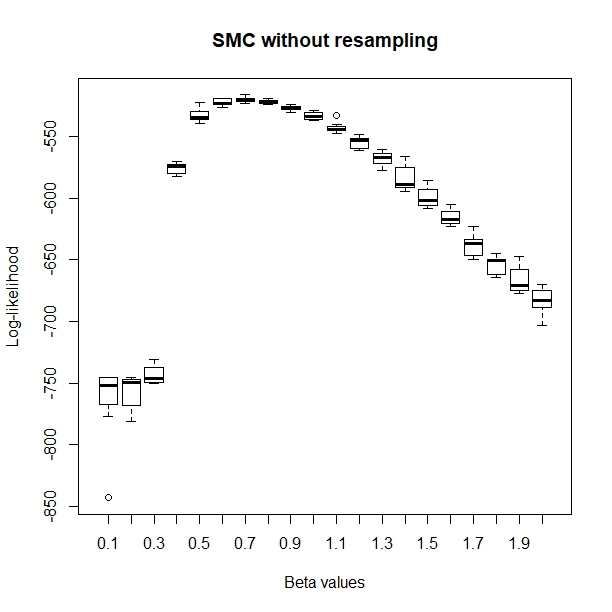
\includegraphics[width=\columnwidth]{task1/SIS_N_10000_T_500.jpeg}
		\caption{Log-likelihood running SIS 10 times, with $N=10^4$ and $T=500$}
	\end{figure}
	The data were generated with the following parameters values: $\phi = 0.97$, $\sigma=0.13$ and $\beta=0.67$. From Figure 1 we can see that the maximum value of the log-likelihood is reached, in mean, for $\beta=0.7$.
	
	\subsection*{Question 2}
	Introducing resampling means to sample from an approximation $\hat{\pi}(x_{1:t})$ which was itself obtained by sampling. We resample $N$ times from $\hat{\pi}(x_{1:t})$, which is equivalent to associating a number of offspring $N_t^i$ with each particle $X_{1:t}^i$ in such a way that $N_t^{1:N} = (N_t^1, ..., N_t^N)$ follow a multinomial distribution with parameter vector $(N, W_t^{1:N})$ and associating a weight of $\frac{1}{N}$ with each offspring. Since we use systematic resampling, the previous algorithm becomes as follows:
	
	Initialization:
	\begin{enumerate}
		\item[-] sample $X_0^i \sim \mathcal{N}(0, \frac{\sigma^2}{1-\phi^2})$
		\item[-] sample $X_1^i \sim \mathcal{N}(\phi x_0^i,\sigma^2) $ 
		\item[-] compute the weights $w_1(X_1^i) = \sum_{j=1}^{N}f(X_1^i|X_0^j)\mu(X_0^j)$ and the normalized weights $W_1(X_1^i)$
		\item[-] compute the incremental weights $ \alpha_1(X_1^i) = g(y_1|X_1^i)w_1(X_1^i) $
		\item[-] sample $U_1 \sim \mathcal{U}[0, \frac{1}{N}]$ and define $U_i = U_1 + \frac{i-1}{N}$
		\item[-] set $N_1^i = |\{ U_j: \sum_{k=1}^{i-1}W_1^k \leq U_j \leq \sum_{k=1}^{i}W_1^k \}|$ with the convention $\sum_{k=1}^{0}=0$, and set the particles to be $N$ equally-weighted of the form $\{\frac{1}{N}, X_1^i\}$
		\item[-] update the values of the incremental weights  $ \alpha_1(X_1^i) $ given the new equally-weighted particles
		\item[-] compute $\log \hat{p}(y_1)$. 
	\end{enumerate}
	Then, at each iteration $t \geq 2$:
	\begin{enumerate}
		\item[-] sample $X_t^i \sim \mathcal{N}(\phi x_{t-1}^i,\sigma^2) $
		\item[-] compute the incremental weights $ \alpha_t(X_{t-1:t}^i) = g(y_t|X_t^i) $
		\item[-] sample $U_1 \sim \mathcal{U}[0, \frac{1}{N}]$ and define $U_i = U_1 + \frac{i-1}{N}$
		\item[-] set $N_t^i = |\{ U_j: \sum_{k=1}^{i-1}W_t^k \leq U_j \leq \sum_{k=1}^{i}W_t^k \}|$ with the convention $\sum_{k=1}^{0}=0$, and set the particles to be $N$ equally-weighted of the form $\{\frac{1}{N}, X_t^i\}$
		\item[-] update the values of the incremental weights  $ \alpha_t(X_{t-1:t}^i) $ given the new equally-weighted particles
		\item[-] compute $\log \hat{p}(y_t|y_{1:t-1})=\log\sum_{i=1}^{N}\frac{1}{N}\alpha_t(X_{t-1:t}^i)$
		\item[-] compute the weights $
		w_t(X_{0:t}^i)=w_0(X_1^i)\prod_{k=2}^{t}\alpha_k(X_{0:k}^i)$ and the normalized weights
	\end{enumerate}
	Considering the same coarse grid for $\beta$, the same data as before, and running 10 times the SMC with resampling for every value of $\beta$, we obtained the result represented in the follwing figure. We ran the SIR algorithm 10 times,  with $N=10^3$ and $T=500$.
	\\
	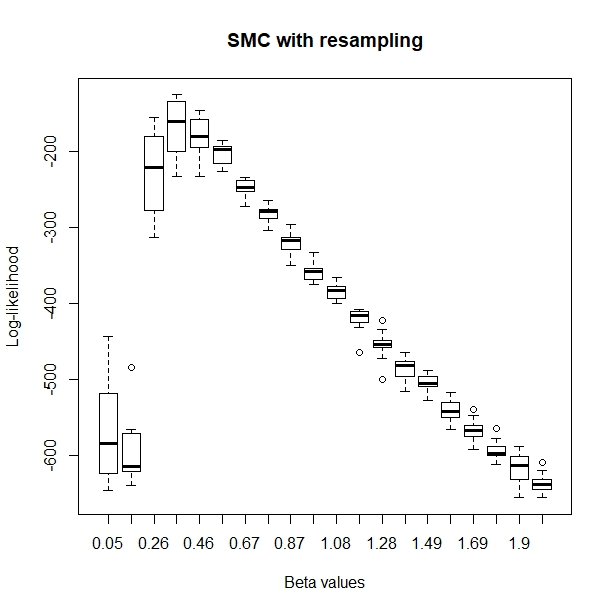
\includegraphics[width=\columnwidth]{task1/SIR_N_1000_T_500.jpeg}
	
	\subsection*{Question 4}
	Finally, we run the algorithm with different values of $T$ and $N$, to study how these parameters affect the variance in the log-likelihood estimate. 
	
	\begin{figure}
		\begin{center}
			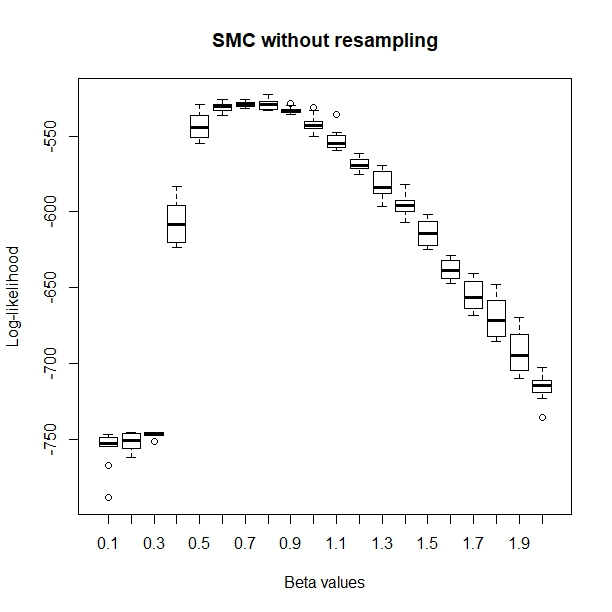
\includegraphics[width=.4\textwidth]{task1/SIS_N_1000_T_500.jpeg}
			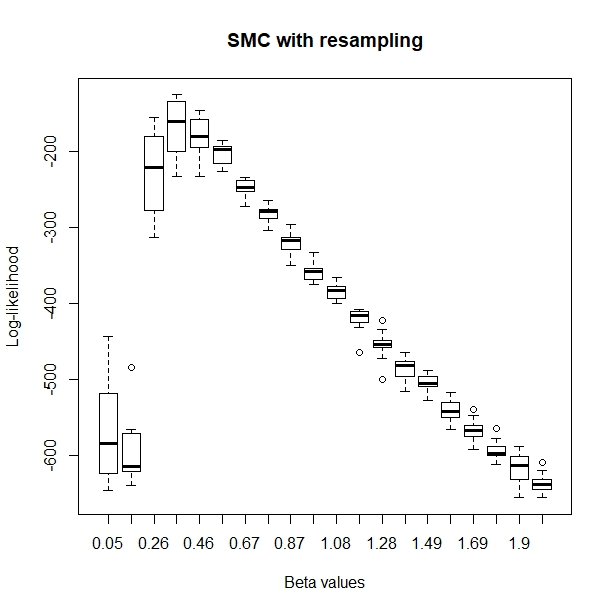
\includegraphics[width=.4\textwidth]{task1/SIR_N_1000_T_500.jpeg}
			\caption*{$N=10^3$ and $T=500$}
			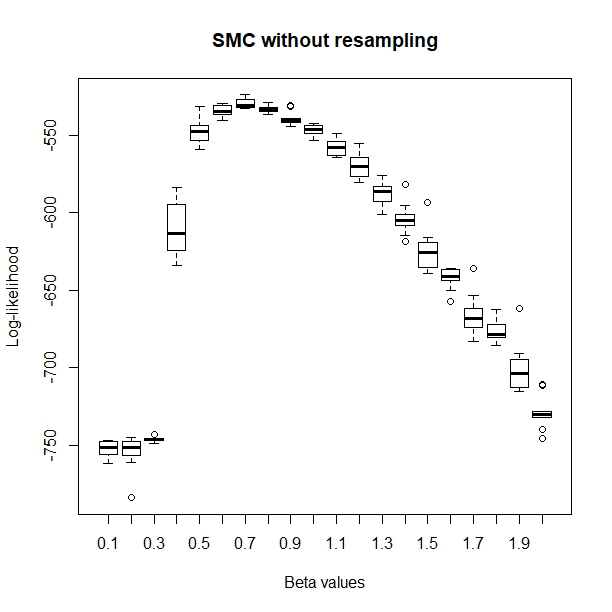
\includegraphics[width=.4\textwidth]{task1/SIS_N_500_T_500.jpeg}
			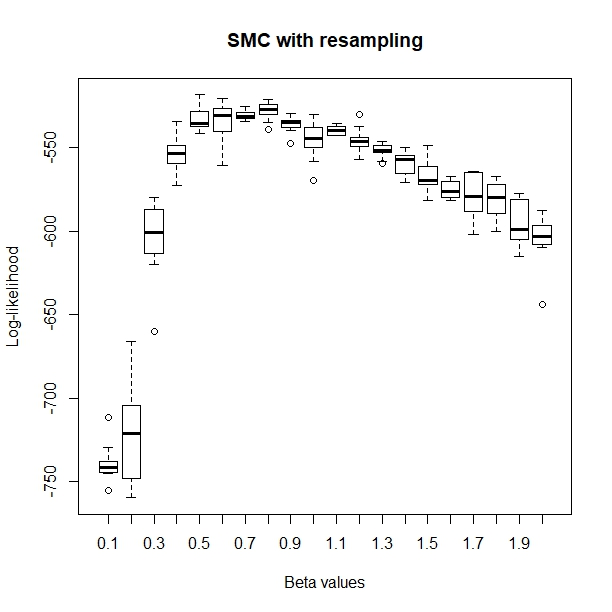
\includegraphics[width=.4\textwidth]{task1/SIR_N_500_T_500.jpeg}
			\caption*{$N=500$ and $T=500$}
			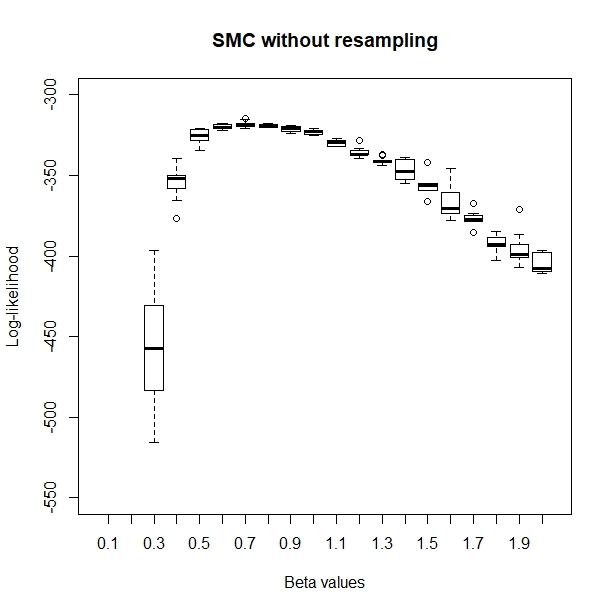
\includegraphics[width=.4\textwidth]{task1/SIS_N_1000_T_300.jpeg}
			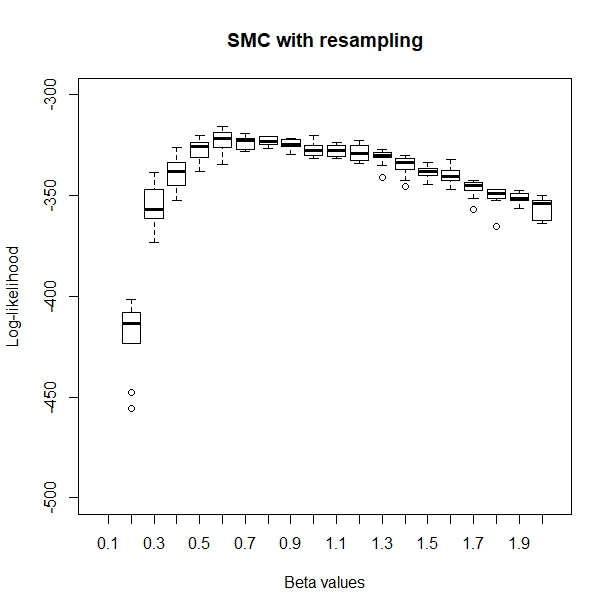
\includegraphics[width=.4\textwidth]{task1/SIR_N_1000_T_300.jpeg}
			\caption*{$N=10^3$ and $T=300$}
		\end{center}
		\caption{Comparison of the results for different values of $T$ and $N$}
	\end{figure}
	
	From Figure 3, we observe that for smaller values of T we have a smaller variance in the estimator, especially in the SMC without resampling. This is due to the fact that for large values of $T$ the particle filtering may degenerate. But, in any case, the SIR algorithm performs better than the SIS one, as we expect. 
	
	\newpage
	
	
	\section*{2.2 MCMC for the stochastic volatility model}
	We will now describe an MCMC sampler for the stochastic volatility model.
	
	1. A time index t is fist sampled uniformly in $\{0, ... , T\}$.
	
	2. Sample $x_t$ from the conditional distribution $p(x_t \mid \theta, x_{0:t-1}, x_{t+1:T},y_{1:T})$, which is given, up to a normalizing constant, by the likelihood function
	
	$ p(x_{0:T}, y_{1:T} \mid \theta) = $
	
	$ \mathcal{N}( x_0 \mid 0, \frac{\sigma^2}{1- \phi^2}) \sum_{t=1}^T [ \mathcal{N}(x_t \mid \phi x_{t-1},\sigma^2 ) \mathcal{N}(y_t \mid 0, \beta^2 exp(x_t))] 
	$
	
	In order to sample $x_t$, use a Metropolis-Hastings sampler characterized by one of the following proposal sampling densities $g_t(x_t' \mid x_t)$ each chosen with probability $1/3$:
	
	1. If $t>0$, sample $ v_n \sim \mathcal{N}(v_n \mid 0,1)$ and set $ x_t' = \phi x_{t-1} + \sigma v_n $ . Otherwise, sample $ x_0' \sim \mathcal{N}(x_0' \mid 0, \frac{\sigma^2}{1- \phi^2})$ .
	2. If $t<T$, sample $ v_n \sim \mathcal{N}(v_n \mid 0,1)$ and set $ x_t' = \frac{x_{t+1} - \sigma v_n}{\phi} $ . Otherwise, set $ x_T' = x_T$ .
	3. If $t>0$, sample $ w_n \sim \mathcal{N}(w_n \mid 0,1)$ and set $ x_t' = 2 log(\frac{|y_t|}{\beta |w_n|}) $ . Otherwise, set $ x_0' = x_0$ .
	
	\textbf{Code path} : ./Codes/task2.2  
	
	\subsection*{Question 6}
	In this task we use Markov Chain Monte Carlo (MCMC) method to generate samples for the distribution $p(x_{0:T}, y_{1:T} \mid \theta)$. In general, the method starts by constructing a Markov chain whose stationary distribution is the target density of interest. 
	
	MCMC method of choice is the Metropolis Hastings algorithm.
	Apart from the distribution we want to sample, the algorithm requires another proposal distribution $g(\mathbf{x'} \mid \mathbf{x})$.
	
	
	Having defined the proposal distribution we start by randomly initializing the initial state $\mathbf{x_0}$. Then we sample a new time step $ t \sim U(0,T)$ which denotes the time step of the stochastic volatility model we sample (not the Monte Carlo time step). 
	
	Next we sample a new $x' \sim g(x' \mid x)$ and compute the acceptance probability $ \alpha = \frac{ \widetilde{p}(x')g(x \mid x') }{  \widetilde{p}(x)g(x' \mid x) }$. If the ratio is higher than one the next state has a higher probability than the previous one and we will always take it, therefore the new acceptance probability is set to 1. Otherwise we want to encourage exploration around the state and we consider taking the next state with the probability $\alpha$.  
	
	\subsubsection*{Initialisation}
	
	The initial state $\mathbf{x_0}$ needs to have a non-zero probability. If this condition isn't met there might be problems with computing the acceptance probability, if the denominator probability is zero acceptance probability is infinite, but that could be reported as a runtime error depending on the programming language and machine we use. The other possibility is that the proposed new state is still in the zero-probability area which would cause a case of $\frac{0}{0}$. Therefore we use Tensorflow framework for function optimization using directed graphs with automatic operation differentiation. We build the computational graph for function:
	
	$ p(x_{0:T}, y_{1:T} \mid \theta) = $
	
	$ \mathcal{N}( x_0 \mid 0, \frac{\sigma^2}{1- \phi^2}) \sum_{t=1}^T [ \mathcal{N}(x_t \mid \phi x_{t-1},\sigma^2 ) \mathcal{N}(y_t \mid 0, \beta^2 exp(x_t))] 
	$
	
	Initialize a random initial state $x_{0:T}$ and use a stochastic gradient descent algorithm to find the **MAP** estimation for the given data $y_{1:T}$.
	
	\subsubsection*{Modeling the proposal density}
	
	Since we are given three different proposal sampling densities, each having the same probability of being chosen, we can construct the following Mixture proposal. We can interpret this as marginalization of a discrete random variable $I$ over three possible classes, one for each function:
	
	$$ g(x' \mid x) = \sum_{k=1}^3 g(x' \mid x, I=i) p(I=i) $$
	
	where $p(I=i)=\frac{1}{3}$ for $ k \in \{ 1,2,3 \}$. 
	
	We then write $ g(x' \mid x, I=i) $ as :
	
	$$ g(x' \mid x, I=i) = g^1(x' \mid x)  \mathbf{1}_{i==1} + g^2(x' \mid x)  \mathbf{1}_{i==2} + g^3(x' \mid x)  \mathbf{1}_{i==3}  $$
	
	where $\mathbf{1}_{L}$ is the indicator function witch results in $1$ if $L$ is true, and in $0$ otherwise. 
	
	Each of $g^i(x' \mid x)$ is a probability density function for the next state $x'$. They are defined as functions of model parameters $\Theta = \{ \sigma, \phi, \beta \}$, predictions $y_{1:T}$, latent variables $x_{0:T}$ and random variables $v_n$ and $w_n$. Therefore, in order to sample from the proposal distribution it is necessary to use the change-of-variable rule for computing the right probability density function and cumulative distribution function needed for the inverse probability transform method of sampling. 
	
	We start with the pdf $g^1(x' \mid x)$. If the selected time step $ t \sim U(0,T)$ turns out to be $0$ we sample from the normal distribution $\mathcal{N}(x_0' \mid 0, \frac{\sigma^2}{1-\phi^2})$. Otherwise we obtain $x_t'$ as:
	
	$$ x_t' = \phi x_{t-1} + \sigma v_n , \quad v_n \sim \mathcal{N}(v_n \mid 0,1) $$
	
	The change-of-variable rule is defined as:
	
	$$ f_Y(y) = \left | \frac{d}{dy} h^{-1}(y) \right | f_X(h^{-1}(y)) \quad \forall y \in g(X)$$
	
	Inverse transformation is:
	
	$$ v_n(x_t') = \frac{1}{\sigma} ( x_t' - \phi x_{t-1})$$
	
	The derivative is :
	
	$$ \frac{d}{d x_t'} v_n(x_t') = \frac{1}{\sigma} $$
	
	And with:
	
	$$  f_{V_n}( x ) = \sqrt{\frac{2}{\pi}} exp\{ -\frac{x^2}{2} \} $$
	
	We obtain:
	
	$$ f_{X_t'}(x_t') = \left | \frac{d}{dx_t'} v_n(x_t') \right | f_{V_n}(v_n(x_t')) $$
	
	$$ f_{X_t'}(x_t') = \frac{1}{\sigma} \sqrt{\frac{2}{\pi}} exp\{ -\frac{(\frac{1}{\sigma} ( x_t' - \phi x_{t-1}))^2}{2} \} $$
	
	$$ f_{X_t'}(x_t') = \frac{1}{\sqrt{2 \pi \sigma}} exp\{ -\frac{( x_t' - \phi x_{t-1})^2}{2 \sigma^2} \} $$
	
	$$ f_{X_t'}(x_t') = \mathcal{N}(x_t' \mid \phi x_{t-1}, \sigma^2) $$
	
	As we have proven, the transformed pdf is also a normal distribution with just a different set of parameters. Rewriting to original notation:
	
	$$ g^1(x' \mid x) = \mathcal{N}(x_t' \mid \phi x_{t-1}, \sigma^2) $$
	
	Putting it all together:
	
	\begin{equation}
	g^1(x' \mid x)=
	\begin{cases}
	\mathcal{N}(x_0' \mid 0, \frac{\sigma^2}{1-\phi^2}), & \text{if}\ t=0 \\
	\mathcal{N}(x_t' \mid \phi x_{t-1}, \sigma^2) , & \text{otherwise}
	\end{cases}
	\end{equation}
	
	$$ f_{X_t'}(x_t') =  \frac{1}{ \sqrt{2 \pi \frac{\sigma^2}{\phi^2} }} exp\{ -\frac{ (\frac{x_{t+1} - \phi x_t'}{\sigma})^2}{2} \}$$
	
	$$ f_{X_t'}(x_t') =  \frac{1}{ \sqrt{2 \pi \frac{\sigma^2}{\phi^2} }} exp\{ -\frac{ ( x_t' - \frac{x_{t+1}}{\phi} )^2}{2 \frac{\phi^2}{\sigma^2}} \}$$
	
	$$ f_{X_t'}(x_t') = \mathcal{N}(x_t' \mid \frac{x_{t+1}}{\phi}, \frac{\phi^2}{\sigma^2}) $$
	
	
	$$ g^2(x' \mid x) = \mathcal{N}(x_t' \mid \frac{x_{t+1}}{\phi}, \frac{\phi^2}{\sigma^2}) $$
	
	
	
	Then, the second case also considers two different distribution with respect to $t \sim U(0,T)$. If the $t = T$ then we just copy the last value to the next: $x_T' = x_T$ .
	Analogous to the first case, the second case will have: 
	
	$$ x_t' =  \frac{( x_{t+1} + \sigma v_n)}{\phi}  , \quad v_n \sim \mathcal{N}(v_n \mid 0,1) $$
	
	Inverse transformation is:
	
	$$ v_n(x_t') = \frac{x_{t+1} - \phi x_t'}{\sigma}  $$
	
	The derivative is :
	
	$$ \frac{d}{d x_t'} v_n(x_t') = -\frac{\phi}{\sigma} $$
	
	And with:
	
	$$  f_{V_n}( x ) = \sqrt{\frac{2}{\pi}} exp\{ -\frac{x^2}{2} \} $$
	
	We obtain:
	
	$$ f_{X_t'}(x_t') = \left | \frac{d}{dx_t'} v_n(x_t') \right | f_{V_n}(v_n(x_t')) $$
	
	$$ f_{X_t'}(x_t') = \left | -\frac{\phi}{\sigma} \right | \sqrt{\frac{2}{\pi}} exp\{ -\frac{ (\frac{x_{t+1} - \phi x_t'}{\sigma})^2}{2} \}$$
	
	$$ f_{X_t'}(x_t') =  \frac{1}{ \sqrt{2 \pi \frac{\sigma^2}{\phi^2} }} exp\{ -\frac{ (\frac{x_{t+1} - \phi x_t'}{\sigma})^2}{2} \}$$
	
	$$ f_{X_t'}(x_t') =  \frac{1}{ \sqrt{2 \pi \frac{\sigma^2}{\phi^2} }} exp\{ -\frac{ ( x_t' - \frac{x_{t+1}}{\phi} )^2}{2 \frac{\phi^2}{\sigma^2}} \}$$
	
	$$ f_{X_t'}(x_t') = \mathcal{N}(x_t' \mid \frac{x_{t+1}}{\phi}, \frac{\phi^2}{\sigma^2}) $$
	
	
	$$ g^2(x' \mid x) = \mathcal{N}(x_t' \mid \frac{x_{t+1}}{\phi}, \frac{\phi^2}{\sigma^2}) $$
	
	
	
	\begin{equation}
	g^2(x' \mid x)=
	\begin{cases}
	\mathcal{N}(x_t' \mid \frac{x_{t+1}}{\phi}, \frac{\phi^2}{\sigma^2}), & \text{if}\ t<T \\
	x_T , & \text{otherwise}
	\end{cases}
	\end{equation}
	
	Finally for the third function we have the flowing rules. If the sampled $t \sim U(0,T)$ is equal to $0$ we set $x_0' = x_0$. Otherwise we have the following function:
	
	$$ x_t' =  2 log(\frac{|y_t|}{\beta |w_n|})  , \quad w_n \sim \mathcal{N}(w_n \mid 0,1) $$
	
	Inverse transformation is:
	
	$$ w_n(x_t') = \left| \frac{|y_t|}{\beta} exp \{ - \frac{x_t'}{2}\} \right | $$
	
	Which is positive on the whole domain so we can exclude the absolute function ( $y_t$ is already required to be absolute and $beta>0$ by definition).
	
	
	The derivative is :
	
	$$ \frac{d}{d x_t'} w_n(x_t') = -\frac{y_t}{2\beta} exp \{ - \frac{x_t'}{2}\} $$
	
	And with:
	
	$$  f_{|W_n|}( x ) = \frac{2}{\sqrt{2 \pi}}  exp\{ -\frac{x^2}{2} \} \quad \forall x \in [0,\inf)$$
	
	Note that here our interval is restricted to only positive numbers, so therefore we need to correct for it in the pdf by multiplying the current value with $2$.
	
	We obtain:
	
	$$ f_{X_t'}(x_t') = \left | \frac{d}{dx_t'} w_n(x_t') \right | f_{W_n}(w_n(x_t')) $$
	
	$$ f_{X_t'}(x_t') = \left | -\frac{y_t}{2\beta} exp \{ - \frac{x_t'}{2}\} \right | \frac{2}{\sqrt{2 \pi}}  exp\{ -\frac{(\frac{y_t}{\beta} exp \{ - \frac{x_t'}{2}\})^2}{2} \} $$
	
	$$ f_{X_t'}(x_t') = \frac{|y_t|}{\beta \sqrt{2 \pi}} exp \bigg\{ -\frac{|y_t|^2}{2 \beta^2} exp\{-x_t' \} - \frac{x_t'}{2} \bigg\} $$
	
	
	\begin{equation}
	g^3(x' \mid x)=
	\begin{cases}
	x_0, & \text{if}\ t=0 \\
	\frac{|y_t|}{\beta \sqrt{2 \pi}} exp \bigg\{ -\frac{|y_t|^2}{2 \beta^2} exp\{-x_t' \} - \frac{x_t'}{2} \bigg\}, & \text{otherwise}
	\end{cases}
	\end{equation}
	
	All relevant equations, side by side :
	
	$$ g(x' \mid x) = \sum_{k=1}^3 g(x' \mid x, I=i) p(I=i) $$
	
	---
	
	$$ g(x' \mid x, I=i) = g^1(x' \mid x)  \mathbf{1}_{i==1} + g^2(x' \mid x)  \mathbf{1}_{i==2} + g^3(x' \mid x)  \mathbf{1}_{i==3}  $$
	
	---
	
	\begin{equation}
	g^1(x' \mid x)=
	\begin{cases}
	\mathcal{N}(x_0' \mid 0, \frac{\sigma^2}{1-\phi^2}), & \text{if}\ t=0 \\
	\mathcal{N}(x_t' \mid \phi x_{t-1}, \sigma^2) , & \text{otherwise}
	\end{cases}
	\end{equation}
	
	---
	
	\begin{equation}
	g^2(x' \mid x)=
	\begin{cases}
	\mathcal{N}(x_t' \mid \frac{x_{t+1}}{\phi}, \frac{\phi^2}{\sigma^2}), & \text{if}\ t<T \\
	x_T , & \text{otherwise}
	\end{cases}
	\end{equation}
	
	---
	
	\begin{equation}
	g^3(x' \mid x)=
	\begin{cases}
	x_0, & \text{if}\ t=0 \\
	\frac{|y_t|}{\beta \sqrt{2 \pi}} exp \bigg\{ -\frac{|y_t|^2}{2 \beta^2} exp\{-x_t' \} - \frac{x_t'}{2} \bigg\}, & \text{otherwise}
	\end{cases}
	\end{equation}
	
	
	\subsubsection*{Acceptance probability}
	
	Acceptance probability is given by the ratio:
	
	$$ \alpha = \frac{ \widetilde{p}(x')g(x \mid x') }{  \widetilde{p}(x)g(x' \mid x) }$$
	
	which can be simplified to :
	
	$$ \alpha = \frac{ \widetilde{p}(x')}{  \widetilde{p}(x) }$$
	
	if the proposal distribution is symmetrical. If it is not symmetrical we need to maintain detailed balance (reversibility) of the stationary distribution by including the ratio between proposal distribution probabilities of the previous state and the next state. 
	
	We know that there normal distributions are always symmetric so we only check for the last equation.
	
	By definition, a probability distribution is said to be symmetric if and only if there exists a value $x_0$ such that 
	$$ f(x_0 - \delta) = f(x_0 + \delta) \quad \forall \delta \in I\!R$$
	
	From there with $\frac{|y_t|}{\sqrt{2 \pi \beta^2}} = C_1$ and $ \frac{|y_t|^2}{2 \beta^2} = C_2 $:
	
	$$ C_1 * exp \bigg\{ -C_2 * exp\{-(x_0 - \delta) \} - \frac{x_0 - \delta}{2} \bigg\}  = C_1 * exp \bigg\{ -C_2 * exp\{-(x_0 + \delta) \} - \frac{x_0 + \delta}{2} \bigg\}$$
	
	$$ -C_2 * exp\{-(x_0 - \delta) \} - \frac{x_0 - \delta}{2} = -C_2 * exp\{-(x_0 + \delta) \} - \frac{x_0 + \delta}{2} $$
	
	
	$$ -C_2 * exp\{-(x_0 - \delta) \} + C_2 * exp\{-(x_0 + \delta) \} =  - \frac{x_0 + \delta}{2} + \frac{x_0 - \delta}{2}  $$
	
	$$ C_2 *  e^{-x_0} ( e^{ \delta} - e^{ -\delta } ) = \delta $$
	
	
	$$ e^{-x_0}  =  \frac{\delta}{C_2( e^{ \delta} - e^{ -\delta } )} $$
	$$ x_0 =  - log(\frac{\delta}{C_2( e^{ \delta} - e^{ -\delta } )} ) $$
	$$ x_0 =  log(\frac{C_2( e^{\delta } - e^{ \delta}   )}{ \delta} ) $$
	
	$$ x_0 =  log\Big( \frac{|y_t|^2}{2 \beta^2} \frac{( e^{ \delta} - e^{ -\delta }   )}{ \delta} \Big) $$
	
	The logarithmic function is defined only for non-negative number, therefore:
	
	$$ \frac{( e^{ \delta} - e^{ -\delta }   )}{ \delta} > 0 $$ 
	
	$$ ( e^{ \delta} - e^{ -\delta } > 0 \land \delta >0 ) \lor ( e^{ \delta} - e^{ -\delta } < 0 \land \delta <0 )$$
	
	
	In the first case, if $\delta >0$ then $ e^\delta > e^{-\delta} $ is always true. Analogous is true for the second equation, if the $\delta <0$ then $ e^\delta < e^{-\delta} $ and therefore we can conclude that the given probability density function is symmetric.
	
	$$\frac{|y_t|}{\beta \sqrt{2 \pi}} exp \bigg\{ -\frac{|y_t|^2}{2 \beta^2} exp\{-x_t' \} - \frac{x_t'}{2} \bigg\}$$
	
	\subsubsection*{Experiments}
	
	Below are listed the samples of values $x_{0,T}$ with $T$ being equal to 20. For longer sequences, such as $T=500$, it was impossible to find a good starting point due to the high dimensionality and therefore the optimization process could not perform as needed. Only the first 6 states are plotted. The generated parameters were $\sigma = 0.304 $ , $\beta = 0.118 $, $\phi = 0.980 $ . The burn in parameter was set to 1000 samples after which we compute 10000 acceptable samples.
	
	\begin{figure}[H]
		\begin{center}
			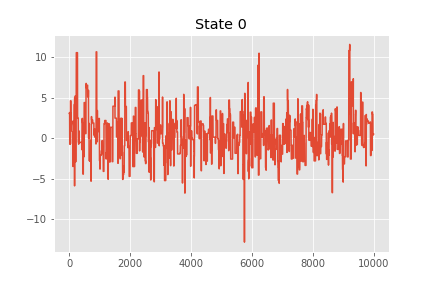
\includegraphics[width=.4\textwidth]{task2/figures/T_2_2/Q1/plt_x0.png}
			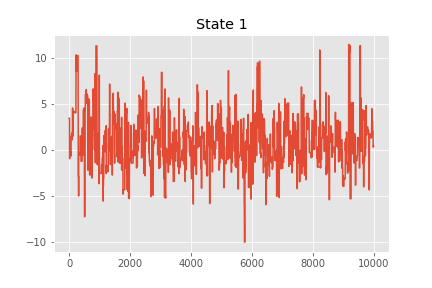
\includegraphics[width=.4\textwidth]{task2/figures/T_2_2/Q1/plt_x1.png}
			
			\caption*{Samples for state $x_0$ and $x_1$}
		\end{center}
	\end{figure}
	
	\begin{figure}[H]
		\begin{center}
			
			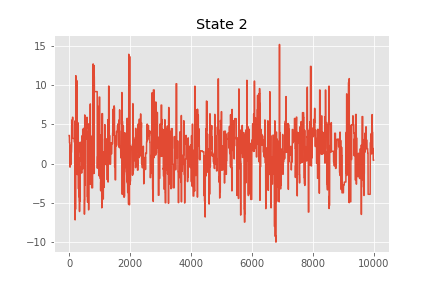
\includegraphics[width=.4\textwidth]{task2/figures/T_2_2/Q1/plt_x2.png}
			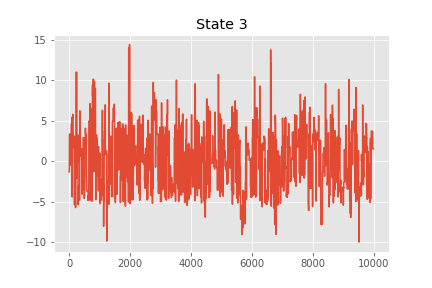
\includegraphics[width=.4\textwidth]{task2/figures/T_2_2/Q1/plt_x3.png}
			
			\caption*{Samples for state $x_2$ and $x_3$}
		\end{center}
	\end{figure}
	
	\begin{figure}[H]
		\begin{center}
			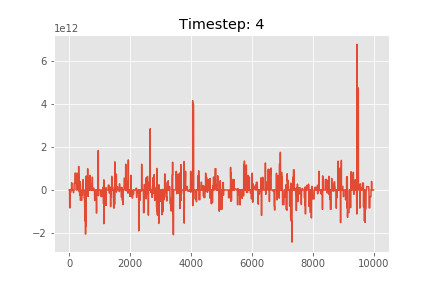
\includegraphics[width=.4\textwidth]{task2/figures/T_2_2/Q1/plt_x4.png}
			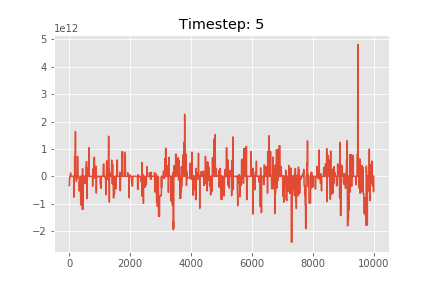
\includegraphics[width=.4\textwidth]{task2/figures/T_2_2/Q1/plt_x5.png}
			
			\caption*{Samples for state $x_4$ and $x_5$}
		\end{center}
	\end{figure}
	
	\begin{figure}[H]
		\begin{center}
			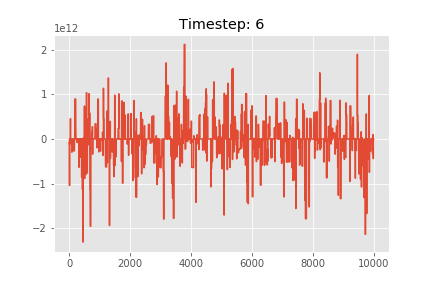
\includegraphics[width=.4\textwidth]{task2/figures/T_2_2/Q1/plt_x6.png}
			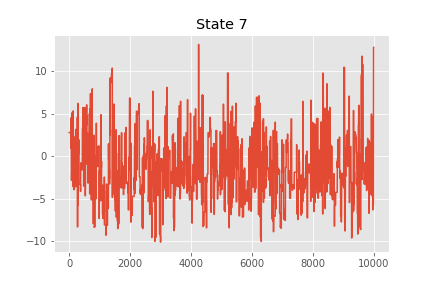
\includegraphics[width=.4\textwidth]{task2/figures/T_2_2/Q1/plt_x7.png}
			
			\caption*{Samples for state $x_6$ and $x_7$}
		\end{center}
	\end{figure}
	
	\begin{figure}[H]
		\begin{center}
			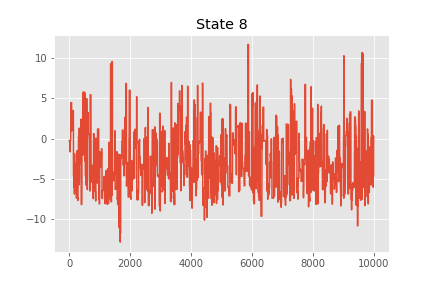
\includegraphics[width=.4\textwidth]{task2/figures/T_2_2/Q1/plt_x8.png}
			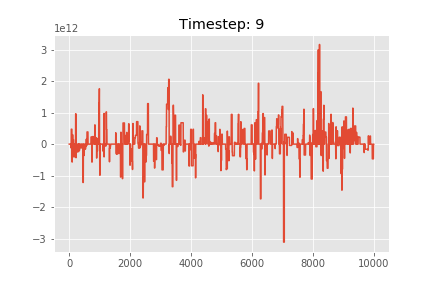
\includegraphics[width=.4\textwidth]{task2/figures/T_2_2/Q1/plt_x9.png}
			
			\caption*{Samples for state $x_8$ and $x_9$}
		\end{center}
	\end{figure}
	
	\begin{figure}[H]
		\begin{center}
			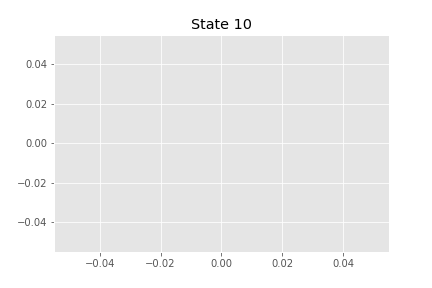
\includegraphics[width=.4\textwidth]{task2/figures/T_2_2/Q1/plt_x10.png}
			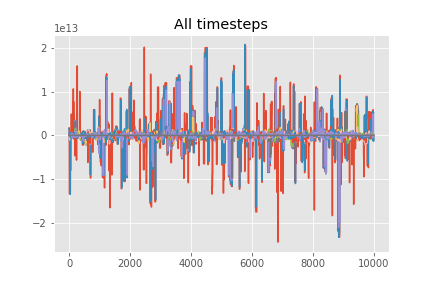
\includegraphics[width=.4\textwidth]{task2/figures/T_2_2/Q1/plt_x_all.png}
			
			\caption*{Samples for state $x_10$ and all the samples on one graph}
		\end{center}
	\end{figure}
	
<<<<<<< HEAD
	\subsubsection*{Question 9}
=======
	\subsubsection{Question 7}
>>>>>>> b2aa0a4ec33d4bc327402c41b10e4b14b0a5734a
	
	For this task the state is extended by two more variables $\sigma^2$ and $\beta^2$ beside the so far used $x_{0:T}$ states. Initially they will be sampled from the Inverse Gamma distribution like follows:
	
	$$ \sigma^2 \sim \mathcal{IG}(a = 0.01, b = 0.01)$$
	$$ \beta^2 \sim \mathcal{IG}(a = 0.01, b = 0.01)$$
	
	
	We will reuse the scheme of sampling uniformly a different variable at each time step but now including the mentioned paramters. The proposed distributions are as follows :
	
	$$ p(\sigma^2 \mid \phi, x_{0:T}, y_{1:T} ) = \mathcal{IG} \left( \sigma^2 \mid a+\frac{T}{2}, b + \frac{1}{2} \sum_{t=1}^T (x_t - \phi x_{t-1})^2 \right) $$
	
	$$ p(\beta^2 \mid \phi, x_{0:T}, y_{1:T} ) = \mathcal{IG} \left( \beta^2 \mid a+\frac{T}{2}, b + \frac{1}{2} \sum_{t=1}^T exp(-x_t)y_t^2 \right) $$
	
	The algorithm is now changed so that in each iteration we sample a value sigma, then a value beta and then a uniformly chosen variable $x_{0:T}$. 
	
	The new dataset parameters are $\sigma = 0.125$, $\beta = 0.185 $ and $\phi=0.962$. The $\sigma^2$ and $\beta^2$ histograms are plotted below, as well as the histograms of the hidden states $x_{0:T}$.
	
	\begin{figure}[H]
		\begin{center}
			
			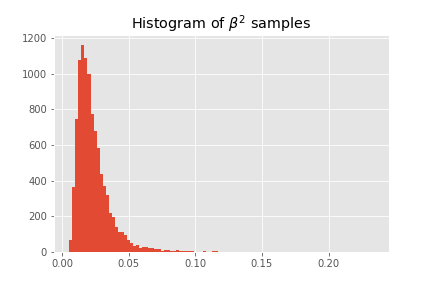
\includegraphics[width=.4\textwidth]{task2/figures/T_2_2/Q2/plt_beta.png}
			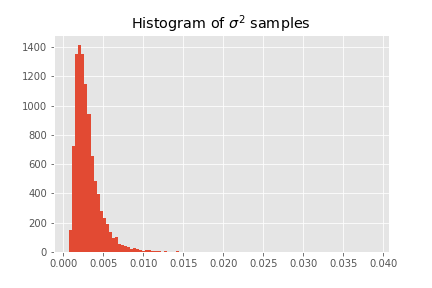
\includegraphics[width=.4\textwidth]{task2/figures/T_2_2/Q2/plt_sigma.png}
			\caption*{Histograms for $\beta^2$ and $\sigma^2$}
		\end{center}
	\end{figure}
	\begin{figure}[H]
		\begin{center}
			
			
			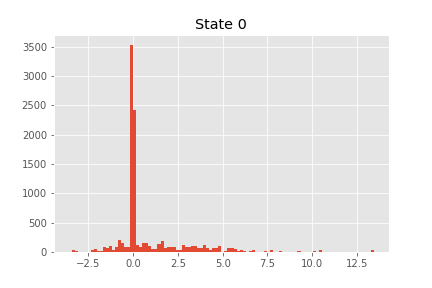
\includegraphics[width=.4\textwidth]{task2/figures/T_2_2/Q2/plt_x0.png}
			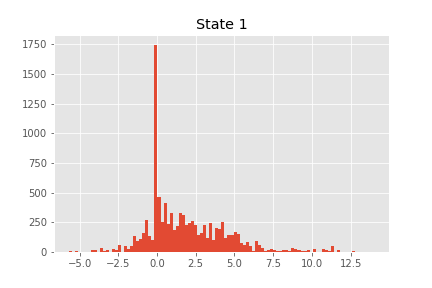
\includegraphics[width=.4\textwidth]{task2/figures/T_2_2/Q2/plt_x1.png}
			
			\caption*{Samples for state $x_0$ and $x_1$}
		\end{center}
	\end{figure}
	\begin{figure}[H]
		\begin{center}
			
			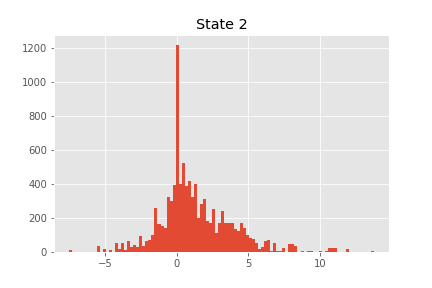
\includegraphics[width=.4\textwidth]{task2/figures/T_2_2/Q2/plt_x2.png}
			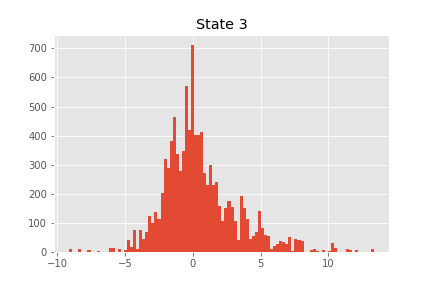
\includegraphics[width=.4\textwidth]{task2/figures/T_2_2/Q2/plt_x3.png}
			
			\caption*{Samples for state $x_2$ and $x_3$}
		\end{center}
	\end{figure}
	\begin{figure}[H]
		\begin{center}
			
			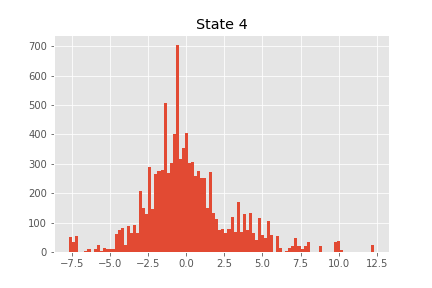
\includegraphics[width=.4\textwidth]{task2/figures/T_2_2/Q2/plt_x4.png}
			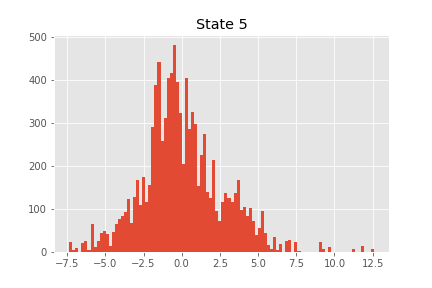
\includegraphics[width=.4\textwidth]{task2/figures/T_2_2/Q2/plt_x5.png}
			
			\caption*{Samples for state $x_4$ and $x_5$}
		\end{center}
	\end{figure}
	\begin{figure}[H]
		\begin{center}
			
			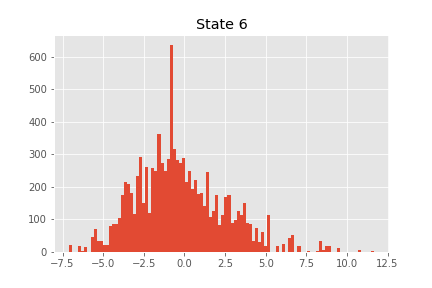
\includegraphics[width=.4\textwidth]{task2/figures/T_2_2/Q2/plt_x6.png}
			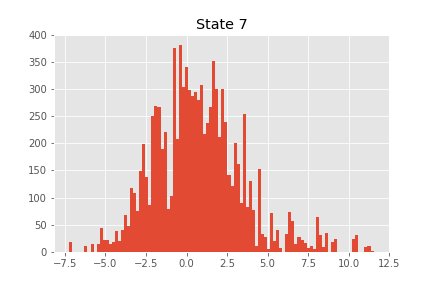
\includegraphics[width=.4\textwidth]{task2/figures/T_2_2/Q2/plt_x7.png}
			
			\caption*{Samples for state $x_6$ and $x_7$}
		\end{center}
	\end{figure}
	\begin{figure}[H]
		\begin{center}
			
			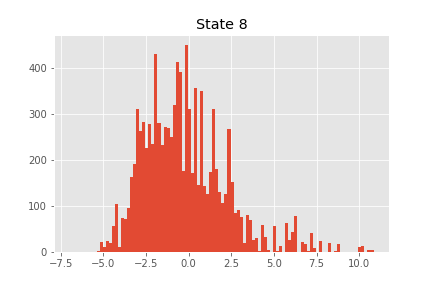
\includegraphics[width=.4\textwidth]{task2/figures/T_2_2/Q2/plt_x8.png}
			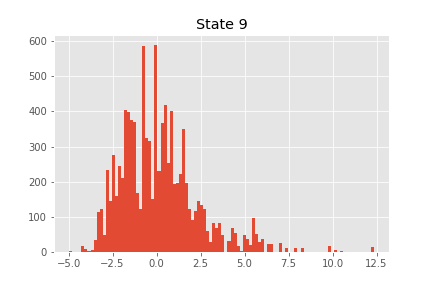
\includegraphics[width=.4\textwidth]{task2/figures/T_2_2/Q2/plt_x9.png}
			
			\caption*{Samples for state $x_8$ and $x_9$}
		\end{center}
	\end{figure}
	\begin{figure}[H]
		\begin{center}
			
			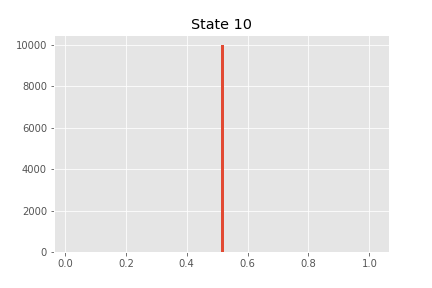
\includegraphics[width=.4\textwidth]{task2/figures/T_2_2/Q2/plt_x10.png}
			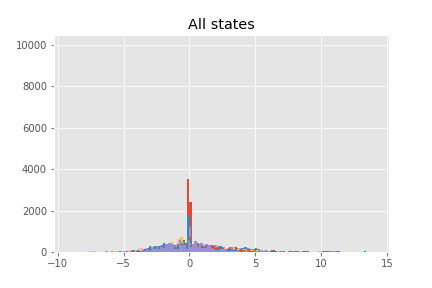
\includegraphics[width=.4\textwidth]{task2/figures/T_2_2/Q2/plt_x_all.png}
			
			\caption*{Samples for state $x_10$ and all the samples on one graph}
			
		\end{center}
	\end{figure}
	
	
	\newpage
	
	
	
	\section*{2.3 MCMC for the train}
	We are given a problem that models a railway with a single train. The map of the tracks is represented by an undirected graph $G=(V,E)$, such that each node has degree 3 and at each vertex edges are labeled $0, L or R$. Each vertex represents a switch: if the train comes from the direction of $L$ or $R$, it always leaves in the direction 0; if the train comes from the direction $0$, it will leave in either direction $L$ or $R$, depending on the state of the switch. The switch has prior probability 1/2 for each direction, but will remain the same throughout the train run. A switch setting is a function $\alpha : V(G) \rightarrow \{L,R\}$
	
	We observe a sequence of $T$ signals, each one representing the label of the edge through which the train has exited a vertex. But the sensors are noisy, and with probability $p = 0.05$, the train reports a random other signal than real direction in which it passed the switch. 
	
	We are given a DP algorithm to compute $p(s,O|G,\alpha)$, where $s=(v,e)$ is called stop position; and the final goal is to estimate the probability distribution of the vector $\alpha(\mathbf{v}) = (\alpha(v_1), ..., \alpha(v_N))$,  where $ N=|V(G)| $, using MCMC.
	
	\textbf{Code path} : ./Codes/task2.3  
	
	\subsection*{Question 8}
	We implemented the class $Graph$ to generate the map of the railway. This class has the following attributes:
	\begin{enumerate}
		\item[-] $V$, the number of nodes 
		\item[-] the degree of the graph ($degree=3$ in our setting) 
		\item[-] $A$, the adjacency matrix, where $A_{ij}=1$ if edge $(i,j)$ exists and $A_{ij}=0$ otherwise
		\item[-] $G$, the matrix representing the labels of the edges, where $G_{ij} \ \in \ \{ 0,1,2,3\} $. We used the convention that 0 represents 0, 1 represents $L$, 2 represents $R$ and 3 is assigned to edges that do not exist.
	\end{enumerate} 
	The map is created randomly, being sure that each vertex has degree 3 and assigning the 3 different labels to the existing edges.
	
	The class $Train$ actually represents our setting: it has a graph, the map; the vector of obervations $O$ and the associated $path$. Observations are generated randomly and, in the end, some noise is added.
	
	In the MCMC Metropolis Hastings algorithm that we propose, states are switch settings vectors and, at each step, the algorithm performs the following operations:
	\begin{enumerate}
		\item[-] propose a new switch setting vector, by simply picking a random vertex and changing its setting. The candidate new state is chosen in this way since we have no particular assumptions and we decided to consider a uniform proposal distribution;
		\item[-] accept the new switch setting with acceptance probability 
		$$
		r(\mathbf{\alpha}_{new}|\mathbf{\alpha}_{old}) = min\{1, a(\mathbf{\alpha}_{new}|\mathbf{\alpha}_{old})\},
		$$
		where
		$$
		a(\mathbf{\alpha}_{new}|\mathbf{\alpha}_{old}) = \frac{p^*(\mathbf{\alpha}_{new})}{p^*(\mathbf{\alpha}_{old})}\frac{q(\mathbf{\alpha}_{old}|\mathbf{\alpha}_{new})}{q(\mathbf{\alpha}_{new}|\mathbf{\alpha}_{old})} 
		$$
		where $p^*$ is the target distribution and $q$ is the proposal distribution, which we assume to be symmetric. So,
		$$
		a(\mathbf{\alpha}_{new}|\mathbf{\alpha}_{old}) = \frac{p(D|\mathbf{\alpha}_{new})}{p(D|\mathbf{\alpha}_{old})} \frac{p(\mathbf{\alpha}_{new})}{p(\mathbf{\alpha}_{old})}
		$$
		Since we have uniform prior for the switch setting of each node and we assume switch settings of different nodes to be independent, and since our data $D$ are given by the vector of observations $\mathbf{O}$ we have
		$$
		a(\mathbf{\alpha}_{new}|\mathbf{\alpha}_{old}) = \frac{p(\mathbf{O}|G,\mathbf{\alpha}_{new})}{p(\mathbf{O}|G,\mathbf{\alpha}_{old})}
		$$
		The probability $p(\mathbf{O}|G,\mathbf{\alpha})$ can be computed using the DP algorithm provided, since it suffices to sum over the all possible stop positions, given particular switch settings. 
	\end{enumerate}
	At the end we obtain sample switch settings, that we store just after the $burn-in$ phase, and their associated probability.
	
	\subsection*{Question 9}
	To run the program, we set $V=6$ and $O=6$. We decided not to consider too many nodes, since otherwise the probabilities associated to the switch setting vectors would have been very small. Setting $V=6$ we expect to understand the results of the MCMC algorithm. Furthermore, first we considered $N=10^3$, that leads to have $10^3$ samples that will actually be considered in the results, and $500$ initial iterations that will be considered as belonging to the \emph{burn-in} phase. The result that we obtained is the following:
	\begin{center}
		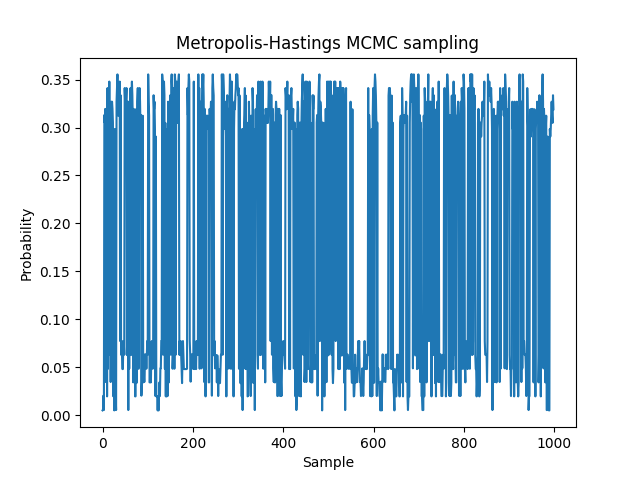
\includegraphics[height=7cm]{task3/V_6_T_6_N_1000.png}
	\end{center}
	We can observe that the probability distribution provided by the sampling is quite stable.
	
	To understand the accuracy of the method, we compared the true switch settings with the most likely, according to the result. The most likely switch settings are the ones that were chosen most often during the sampling. 
	\begin{center}
		\begin{tabular}{| c | c | c | c | c | c | c |}
			True $\alpha(\mathbf{v})$ & $R$ & $L$ & $L$ & $R$ & $R$ & $L$ \\
			ML $\alpha(\mathbf{v})$ & $R$ & $L$ & $R$ & $R$ & $R$ & $L$ \\
		\end{tabular}
	\end{center}
	In particular, we provide the plot of the MCMC Metropolis Hastings label proposals for node 1.
	\begin{center}
		\begin{tabular}{| c |}
			$p(\alpha(v_1)=L) = 0.46 $ \\
			$p(\alpha(v_1)=R) = 0.54 $ \\
		\end{tabular}
	\end{center}
	\begin{center}
		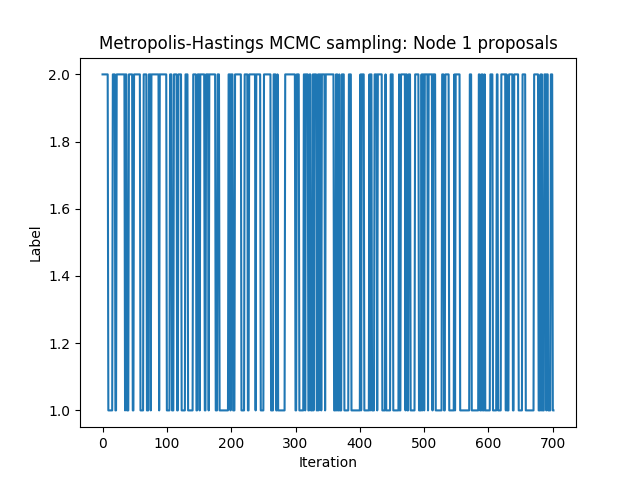
\includegraphics[height=6.8cm]{task3/V_6_T_6_N_1000_Node1.png}
	\end{center}
	Running again the program, performing $N=10^4$ iterations, we have the following results:
	\begin{center}
		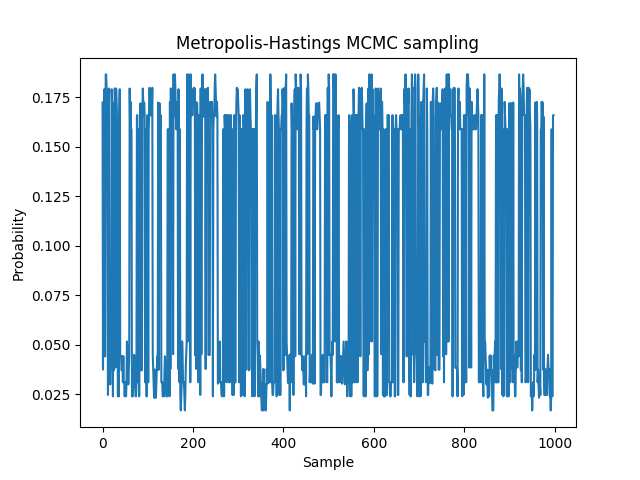
\includegraphics[height=7cm]{task3/V_6_T_6_N_10000.png}
		\begin{tabular}{| c | c | c | c | c | c | c |}
			True $\alpha(\mathbf{v})$ & $R$ & $R$ & $L$ & $L$ & $R$ & $R$ \\
			ML $\alpha(\mathbf{v})$ & $R$ & $R$ & $L$ & $R$ & $R$ & $L$ \\
		\end{tabular}
		\\
		\begin{tabular}{| c |}
			$p(\alpha(v_1)=L) = 0.51 $ \\
			$p(\alpha(v_1)=R) = 0.49 $ \\
		\end{tabular}
	\end{center}
	Note that in the plots we show just the last $10^3$ iterations to make them more clear to the reader. 
	
	\subsection*{Question 10}
	Now, we aim to perform the same analysis using Gibbs sampling instead of Metropolis Hastings. So, at each iteration $i = 1...N$
	\begin{enumerate}
		\item[-] sample $\alpha(v_1)$, 
		\item[-] sample $\alpha(v_2)$,
		\item[-] ...
		\item[-] sample $\alpha(v_V)$,  
	\end{enumerate} 
	In particular, for each node $j \in V(G)$, the sampling step is done according to
	$$
	\text{with probability } \frac{1}{2} \text{, } \alpha(v_j^{i+1}) = \alpha(v_j^i)
	$$
	$$
	\text{with probability } \frac{1}{2} \text{, } \alpha(v_j^{i+1}) \neq \alpha(v_j^i)
	$$
	Setting $V=6$, $T=6$ and $N=10^4$, we obtained
	\begin{center}
		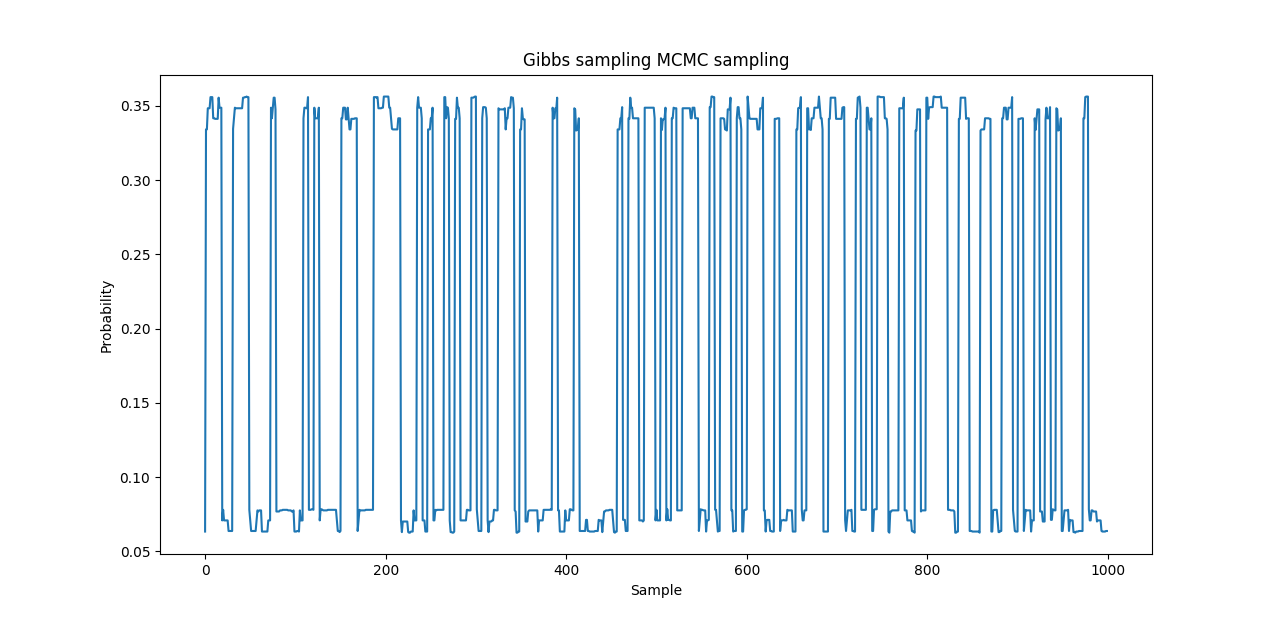
\includegraphics[width=\columnwidth]{task3/V_6_T_6_N_10000_Gibbs.png}
		\begin{tabular}{| c | c | c | c | c | c | c |}
			True $\alpha(\mathbf{v})$ & $R$ & $R$ & $L$ & $L$ & $R$ & $R$ \\
			ML $\alpha(\mathbf{v})$ & $R$ & $R$ & $R$ & $L$ & $L$ & $R$ \\
		\end{tabular}
	\end{center}
	Considering blocked Gibbs sampling, we can say that the Metropolis Hasting algorithm proposed in the previous part of the task corresponds to blocked Gibbs with blocked size equal to $V$, since in MH we change randomly one component of the switch setting vector at each iteration. We could consider any size for blocked Gibbs: if we consider $n \leq V$ ($n > 1$) groups of components at each iteration, then we change randomly $n$ switch settings of $\alpha(\mathbf{v})$.
	
	For instance, we run the blocked Gibbs sampling for $n=2$ with $V=6$, that means that we consider at each iteration 3 groups of components. We obtained a more accurate result:
	\begin{center}
		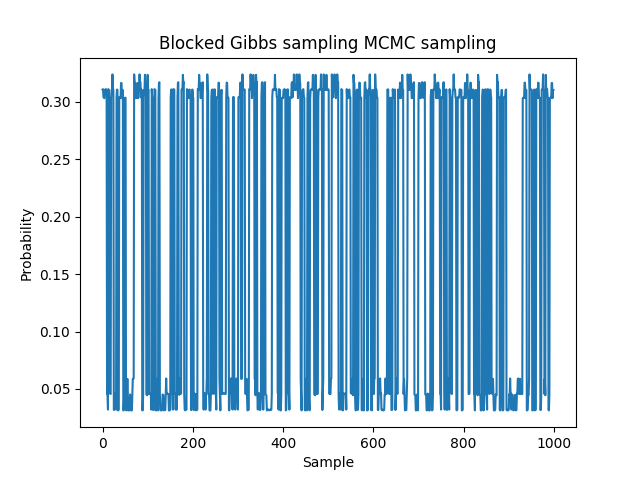
\includegraphics[height=6cm]{task3/V_6_T_6_N_10000_Blocked_Gibbs.png}
		\begin{tabular}{| c | c | c | c | c | c | c |}
			True $\alpha(\mathbf{v})$ & $L$ & $R$ & $L$ & $R$ & $R$ & $R$ \\
			ML $\alpha(\mathbf{v})$ & $L$ & $R$ & $L$ & $R$ & $R$ & $R$ \\
		\end{tabular}
	\end{center}
	
	In our sampling algorithms we do not need to sample the stop position $s$ for the reasoning about proposals and acceptance probabilities that we provided at the beginning of the task. However, we could compute the probability associated to each stop position given the switch settings. 
	
	\newpage
	
	\section*{2.4 Gibbs sampler for the magic word}
	
	The following generative model magic word generates $N$ sequences if length $M$, $s^1, ..., s^N $ where $s^n = s_1^n, ... ,s_M^n $. All sequences are over the alphabet $[K]$. Each of these sequences has a "magic" word of length W hidden in it and the rest of the sequence is called background. 
	
	First, for each $n$, a start position $r_n$ for the magic word is sampled uniformly from $[M-w+1]$. Then the $j$:th positions in the word are sampled from $q_j(x)=Cat(x \mid \theta_j)$ where $\theta_j$ has a $Dir( \theta_j \mid \alpha)$ prior. All other positions in the sequences are sampled from the background distribution $q(x) = Cat(x \mid \theta)$ where $\theta$ has a $Dir(\theta \mid \alpha') prior.$
	
	We are interested in the posterior $p(r_1,...,r_N \mid D)$ where $D$ is the set of sequences $ s^1, ..., s^N$ generated by the model and the $r_n$ is the start position of the magic word in the $n$:th sequence $s^n$. The following describes a Gibbs sampler that can be used for estimating the posterior over start positions after having observed $s^1, ..., s^N$. The sampler that can be used for estimating the posterior over start positions and $\alpha'$. The states are vectors of start position $R= (r_1,...,r_N)$
	
	Notice that, for the Dirichlet-categorical (Dirichlet-multinoulli) distribution for the $j$:th position of the magic words, the marginal likelihood is 
	
	$$ p(D_j \mid R) = \frac{\Gamma(\sum_k \alpha_k)}{\Gamma(N \sum_k \alpha_k)} \prod_k \frac{\Gamma( N_k^j + \alpha_k)}{\Gamma(\alpha_k)} $$
	
	where $N_k^j$ is the count of the symbol $k$ in the $j$:th column of the magic words, introduced by $R$. For the background, the marginal likelihood is 
	
	$$ p(D_B \mid R) = \frac{\Gamma(\sum_k \alpha_k')}{\Gamma(B \sum_k \alpha_k')} \prod_k \frac{\Gamma( B_k + \alpha_k')}{\Gamma(\alpha_k')} $$
	
	where $B$ is the number of background positions (i.e. $N(M-w)$) and $B_k$ is the count of symbol $k$ in the background, induced by $R$. The full condition $p(r_n \mid R_{-n}, D)$ can be expressed as follows
	
	\begin{align*}
	p(r_n \mid R_{-n}, D) &= \frac{p(R_{-n} \cup r_n, D)}{p(R_{-n}, D)} \\
	& \propto p(R_{-n} \cup r_n, D) \\
	& \propto p(D \mid R_{-n} \cup r_n) \\
	& = p(D_B \mid R_{-n} \cup r_n) \prod_j p(D_j \mid R_{-n} \cup r_n)
	\end{align*}
	
	\textbf{Code path} : ./Codes/task2.4  
	
	\subsection*{Question 11}
	
	The task consists of two practical parts: implementing the data generator and implementing the Gibbs sampler. 
	
	Data generator needs to produce $N$ sequences, each of length $M$. Every element in the sequence will be a token over the alphabet of size $K$. In our experiments the alphabet will consist of letters $a,b,c,d$, therefore $K$ being equal to $4$, we'll set $M=30$ and $W=10$. We also set the number of samples $N=10$, Dirichlet prior parameter for background  to vector $\alpha' = [1,1,1,1]$ and the Dirichlet prior parameter for magic word  $\alpha = [12,7,3,1]$ .
	
	The process of generating data starts by generating parameters $\theta'$ and $\theta$ from the Dirichlet priors $\alpha'$ and $\alpha$ respectively. We then sample a background for each sequence using the multinomial distribution with parameter $\theta$. Then we uniformly choose a position of the start of the magic word $p_{mw} \sim U(0, M-W+1)$ and sample for the magic word tokens from multinomial distribution with the parameters $\theta$. 
	
	Next comes the Gibbs sampler which we want to use to find the start positions of the magic words in sequences. We use $r_n$ to denote the start position of the magic word in the $n^{th}$ sequence. Therefore we estimate $p(r_1,...,r_n \mid \mathcal{D})$ where $\mathcal{D}$ is the generated data, i.e. the provided sequences.
	
	The task requires of us to use collapsed Gibbs sampler, which supports scenarios where some of the unknown quantities are analytically integrated. This method is also much more efficient, since it is sampling in a lower dimensional space. In our case $\alpha$ and $\alpha'$ are know parameters but the sequences are sampled from Multinomial distribution of parameter $\theta$, generated from $\alpha'$ used for background symbols and $\theta_j$, generated from $\alpha$ used for magic words symbols per position $j \in [1,..,W]$. Therefore we will integrate out the $\theta$ and $\theta_j$ parameters, which will cause all the symbols in sequences to become inter-dependent.
	
	The initial state $R^{(0)} = r_1^0, ..., r_n^0$ is initialized randomly  and they will be re-sampled in the Gibbs sampling process. 
	
	In each iteration of the sampling process we calculate the probability of each proposed position $r_n^{(i)}$ of being the real starting position of the magic word using:
	
	$$ p(r_n^{(i)} \mid \mathcal{R}_{-n}^{(i)}, \mathcal{D}) \propto p(\mathcal{D}_{B} \mid \mathcal{R}^{(i)}, \alpha') \prod_{j=l}^{l+W} p(\mathcal{D}_j \mid \mathcal{R}^{(i)}, \alpha)$$ 
	
	In the above equation $r_n^{(i)}$ denotes a vector of size $| M-W+1 |$ of probabilities of every valid position being the starting one, for the $n^{th}$ sequence. 
	
	
	In order to get a more numerically stable probability measure we will apply the $log$ function to the probability functions. Distribution for the $j$:th position of the magic words now looks like:
	
	$$ p(D_j \mid R) = \left[log\left(\Gamma(\sum_k \alpha_k) \right) - log\left(\Gamma(N \sum_k \alpha_k)\right) \right] \sum_k \left[ log\left(\Gamma( N_k^j + \alpha_k)\right) - log\left(\Gamma(\alpha_k)\right) \right] $$
	
	where $N_k^j$ is the count of the symbol $k$ in the $j$:th column of the magic words, introduced by $R$. The log-background marginal likelihood is calculated as
	
	$$ p(D_B \mid R) = \left[ log\left(\Gamma(\sum_k \alpha_k') \right) - log\left(\Gamma(B \sum_k \alpha_k')\right) \right] \sum_k \left[ log\left(\Gamma( B_k + \alpha_k')\right) - log\left(\Gamma(\alpha_k') \right) \right] $$
	
	where $B$ is the number of background positions (i.e. $N(M-w)$) and $B_k$ is the count of symbol $k$ in the background, induced by $R$.
	
	
	The generated vector is used as the parameter of the categorical distribution from which we sample the new starting positions $r_n^{(i+1)}$ and we do this through burn-in phase after which we can sample from the target distribution.
	
	\subsection*{Question 12}
	
	To show we attained convergence we will provide to forms of proof: a visual one and a numeric one. 
	
	The full sequence has a length of $M=30$ with the length of magic-word being $M=10$. First we repeat the sampling procedure $C=10$ times in order to obtain $10$ independent randomly initialized chains. Each chain has $500$ samples. We ignore the burn-in in order to observe the full convergence from the initial state in the plots, but the estimated potential scale reduction statistics is computed for last $N=1000$, $N=500$, $N=100$ samples taken from the previously sampled data. 
	
	The true position are as follows:
	
	\begin{center}
		\begin{tabular}{||c c c c c c c c c c||} 
			\hline
			p1 & p2 & p3 & p4 & p5 & p6 & p7 & p8 & p9 & p10 \\ [0.5ex] 
			\hline\hline
			17 & 8 & 1 & 3 & 1 & 12 & 19 & 16 & 1 & 5 \\ [1ex]
			\hline
		\end{tabular}
	\end{center}
	
	The next series of plots represent the sampled positions over time for each chain.
	We observe that the chain converges to good points quickly or it gets stuck between a few similar values. 
	
	\begin{figure}[H]
		\begin{center}
			
			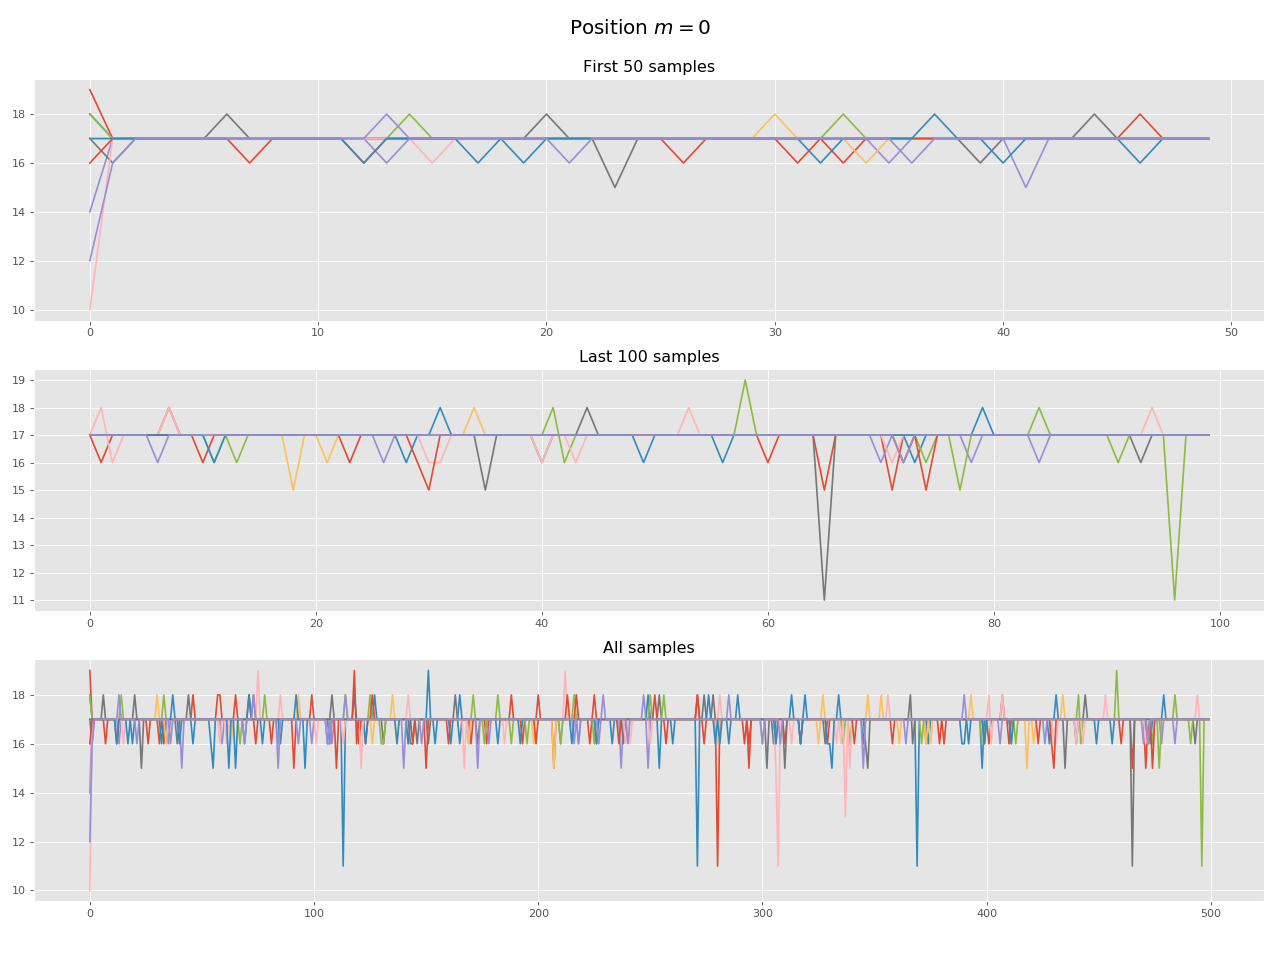
\includegraphics[width=.7\textwidth]{task4/figures/T_2_4/Q2/convergence_pos0.png}
			\caption*{Samples for position 0}
		\end{center}
	\end{figure}
	
	\begin{figure}[H]
		\begin{center}
			
			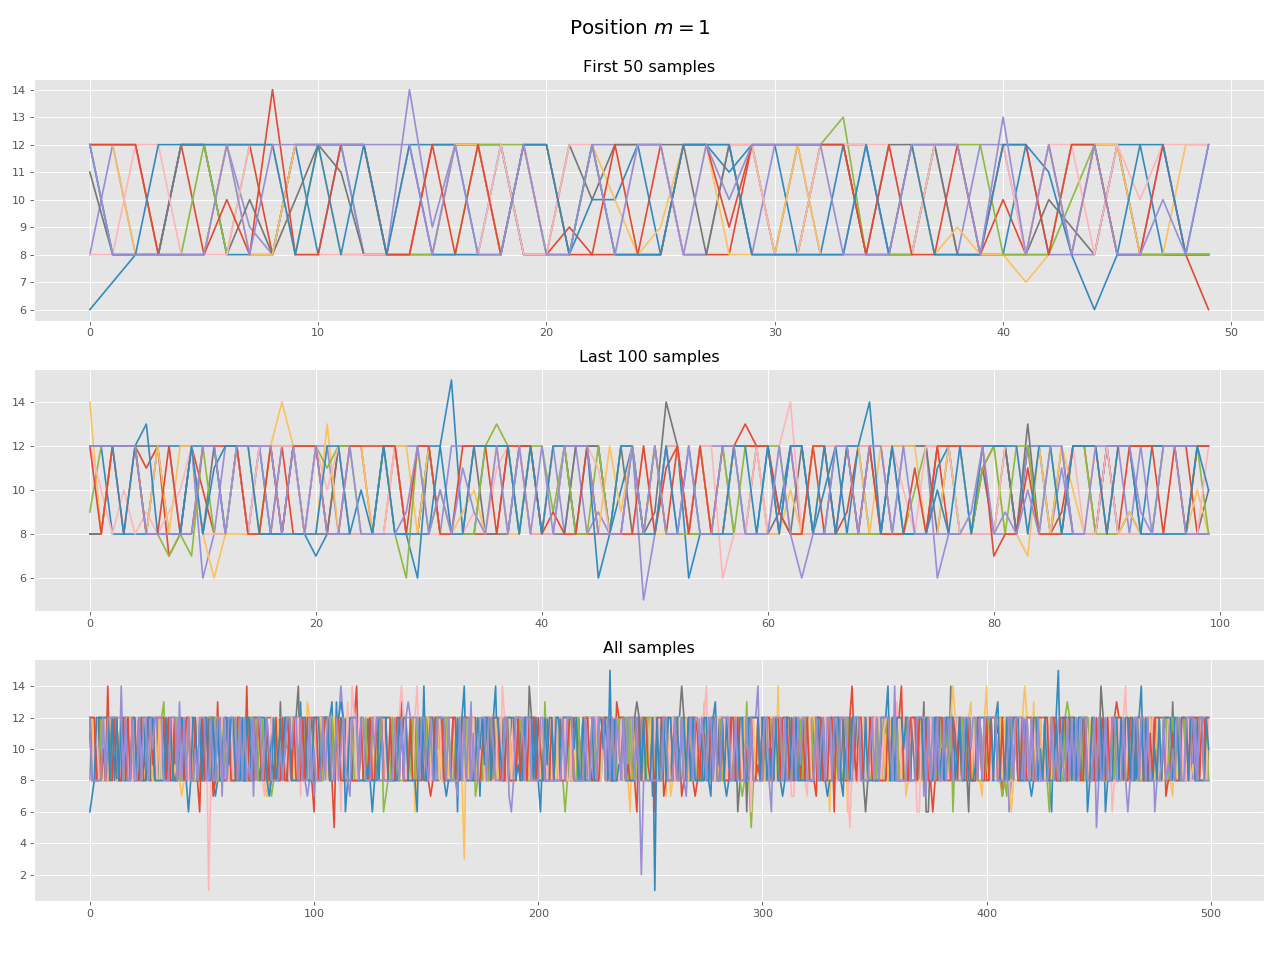
\includegraphics[width=.7\textwidth]{task4/figures/T_2_4/Q2/convergence_pos1.png}
			\caption*{Samples for position 1}
		\end{center}
	\end{figure}
	
	\begin{figure}[H]
		\begin{center}
			
			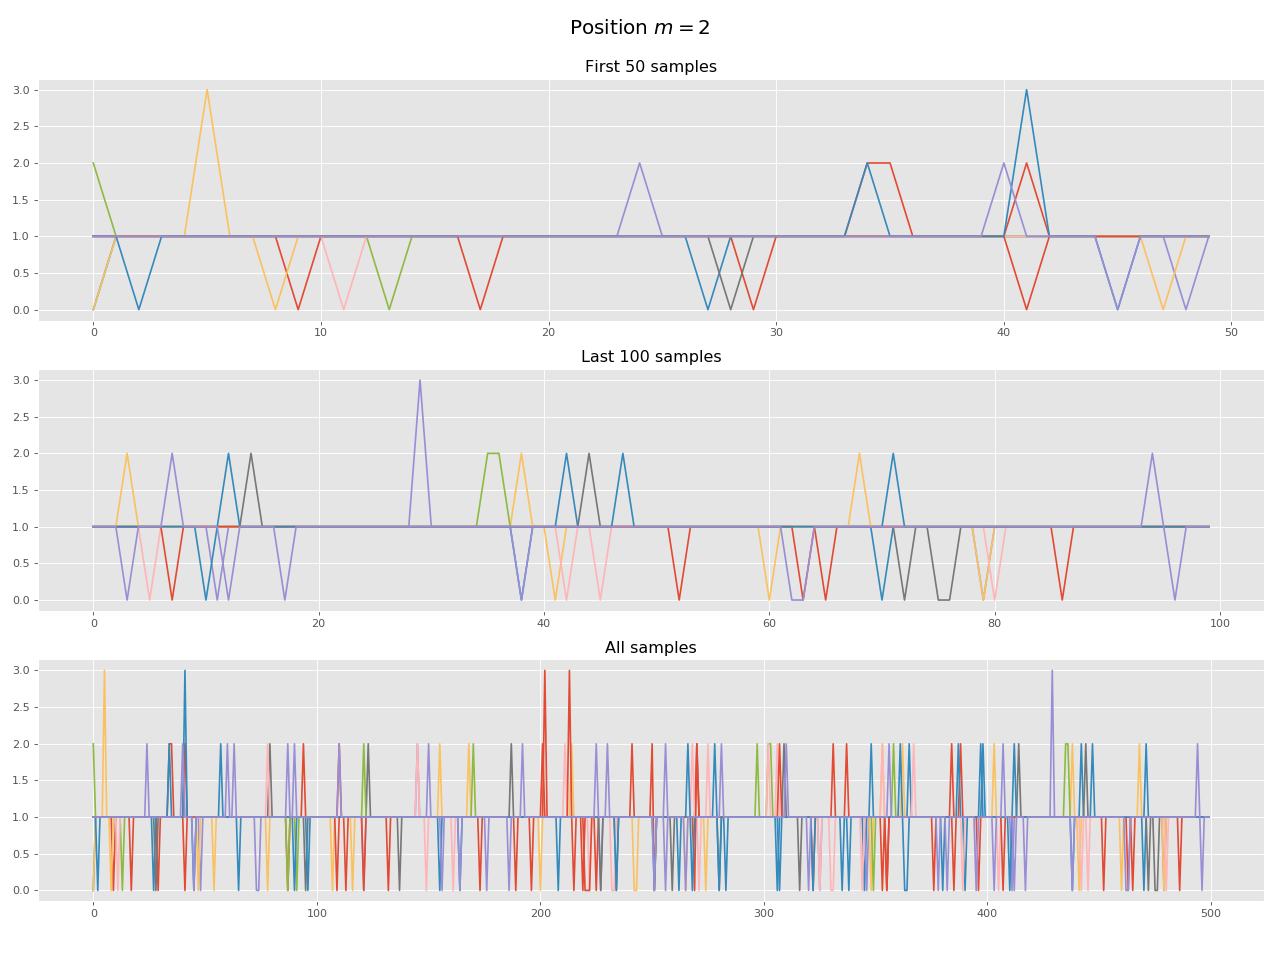
\includegraphics[width=.7\textwidth]{task4/figures/T_2_4/Q2/convergence_pos2.png}
			\caption*{Samples for position 2}
		\end{center}
	\end{figure}
	
	\begin{figure}[H]
		\begin{center}
			
			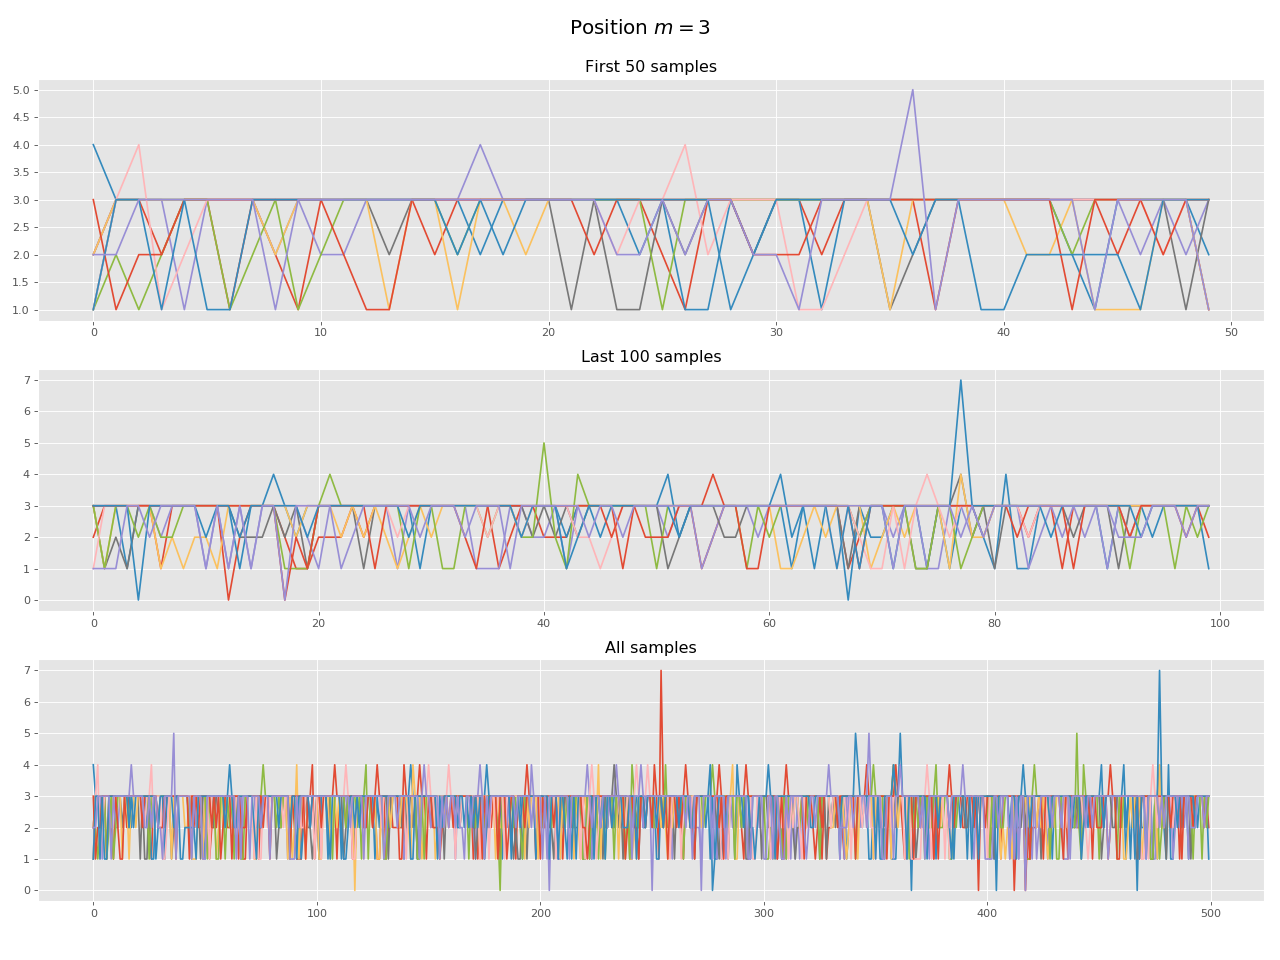
\includegraphics[width=.7\textwidth]{task4/figures/T_2_4/Q2/convergence_pos3.png}
			\caption*{Samples for position 3}
		\end{center}
	\end{figure}
	
	\begin{figure}[H]
		\begin{center}
			
			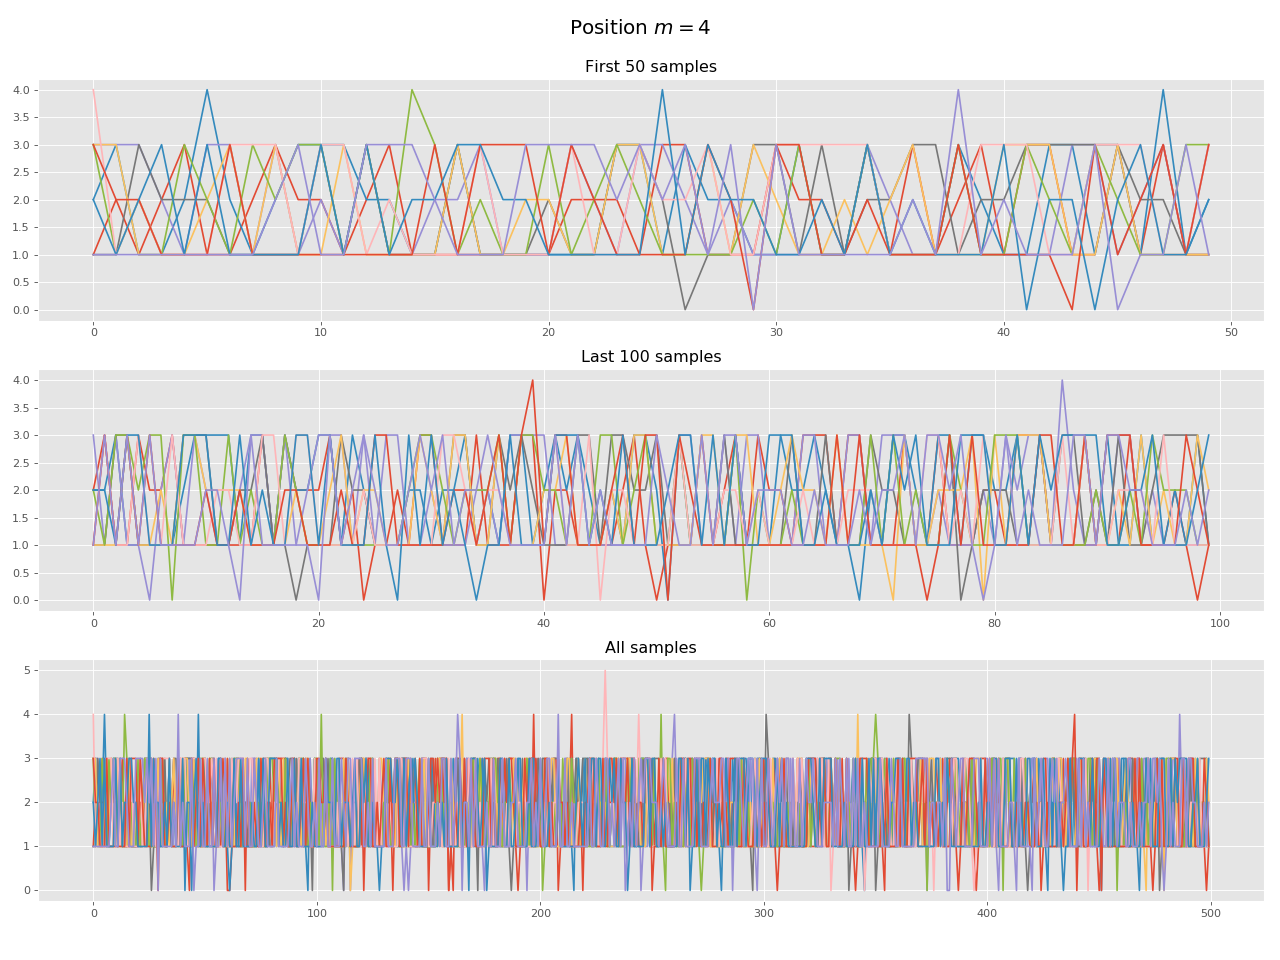
\includegraphics[width=.7\textwidth]{task4/figures/T_2_4/Q2/convergence_pos4.png}
			\caption*{Samples for position 4}
		\end{center}
	\end{figure}
	
	\begin{figure}[H]
		\begin{center}
			
			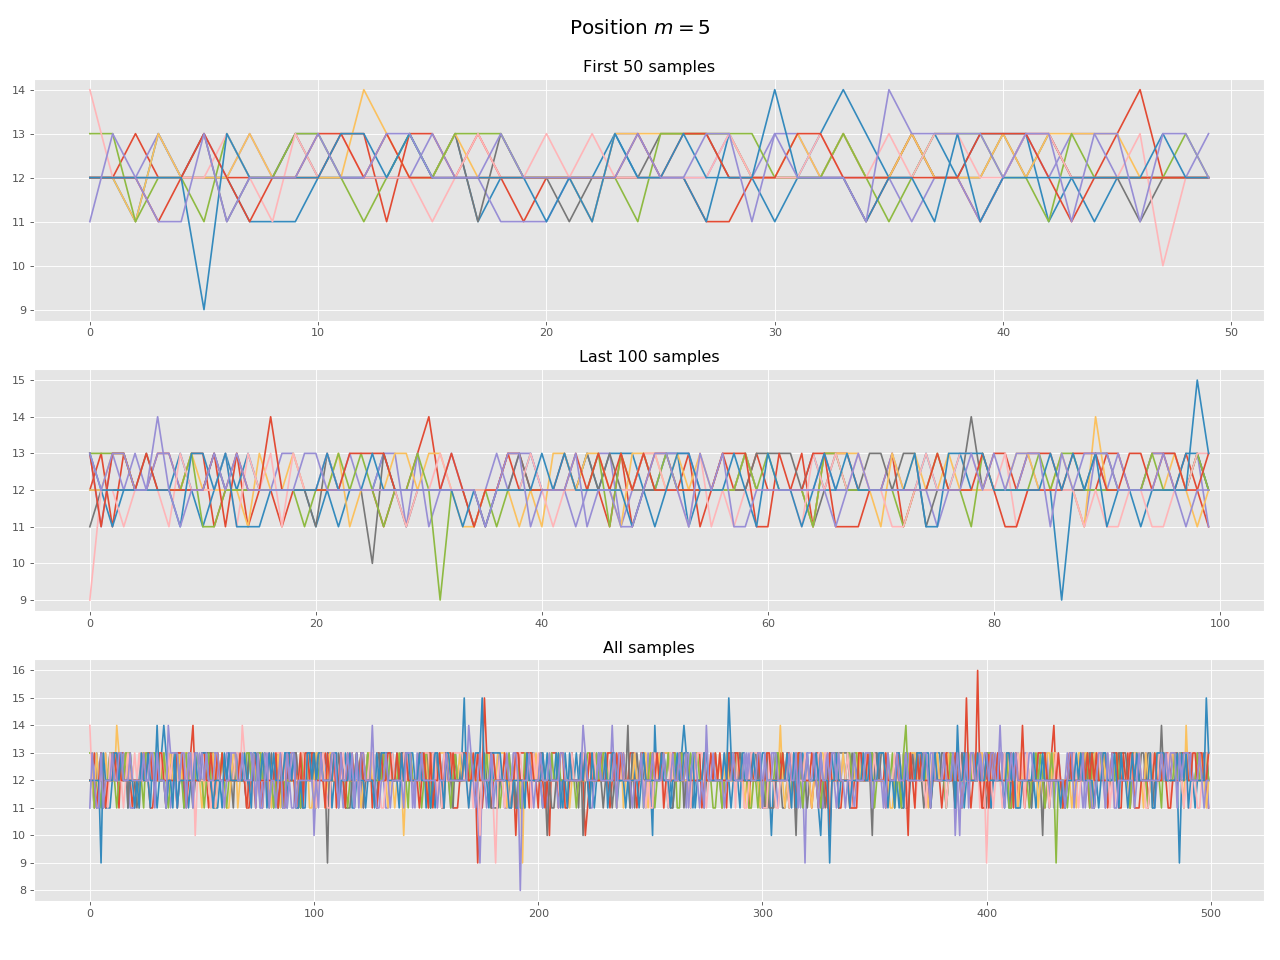
\includegraphics[width=.7\textwidth]{task4/figures/T_2_4/Q2/convergence_pos5.png}
			\caption*{Samples for position 5}
		\end{center}
	\end{figure}
	
	\begin{figure}[H]
		\begin{center}
			
			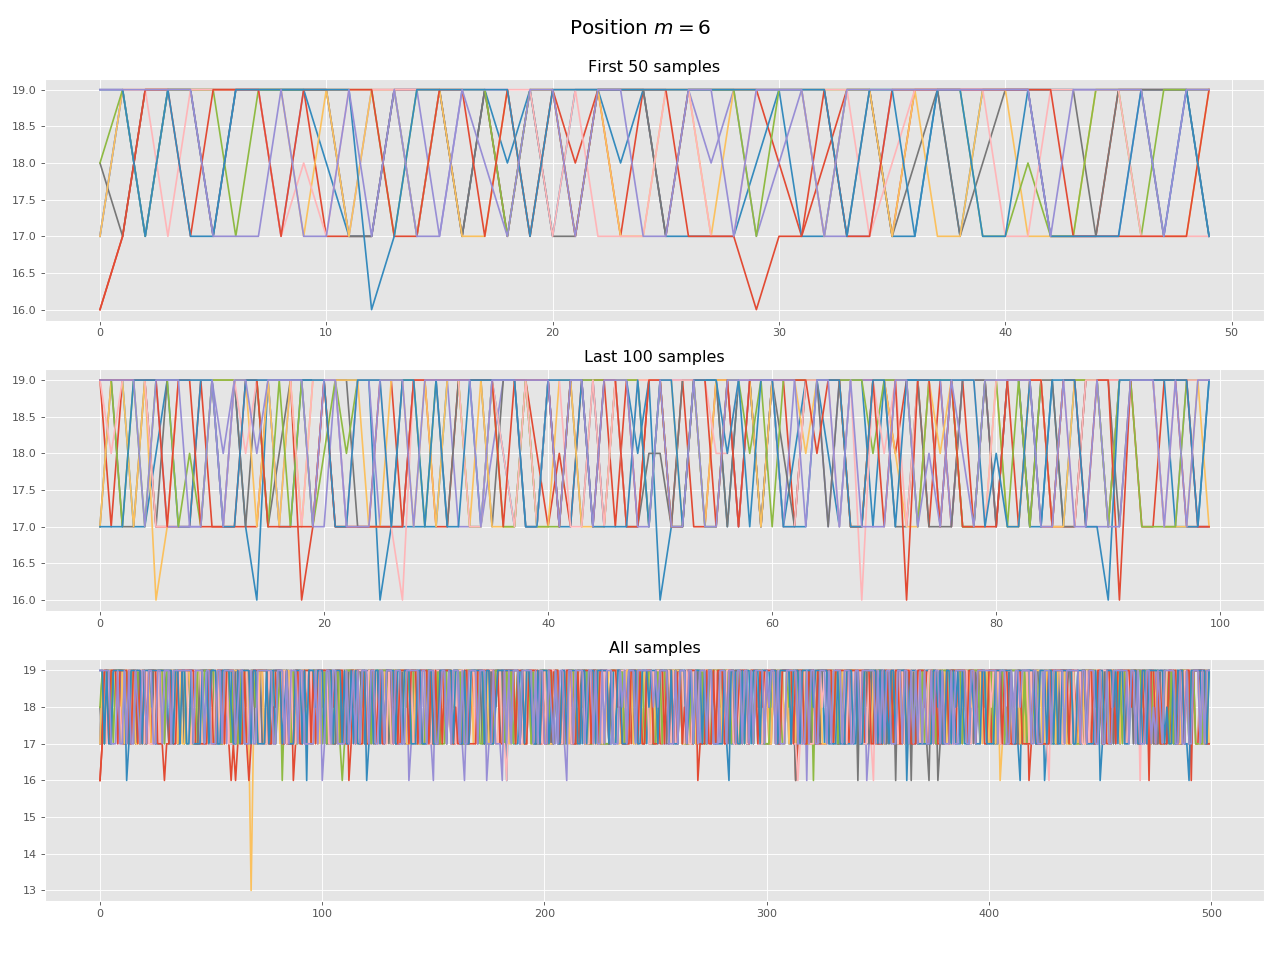
\includegraphics[width=.7\textwidth]{task4/figures/T_2_4/Q2/convergence_pos6.png}
			\caption*{Samples for position 6}
		\end{center}
	\end{figure}
	
	\begin{figure}[H]
		\begin{center}
			
			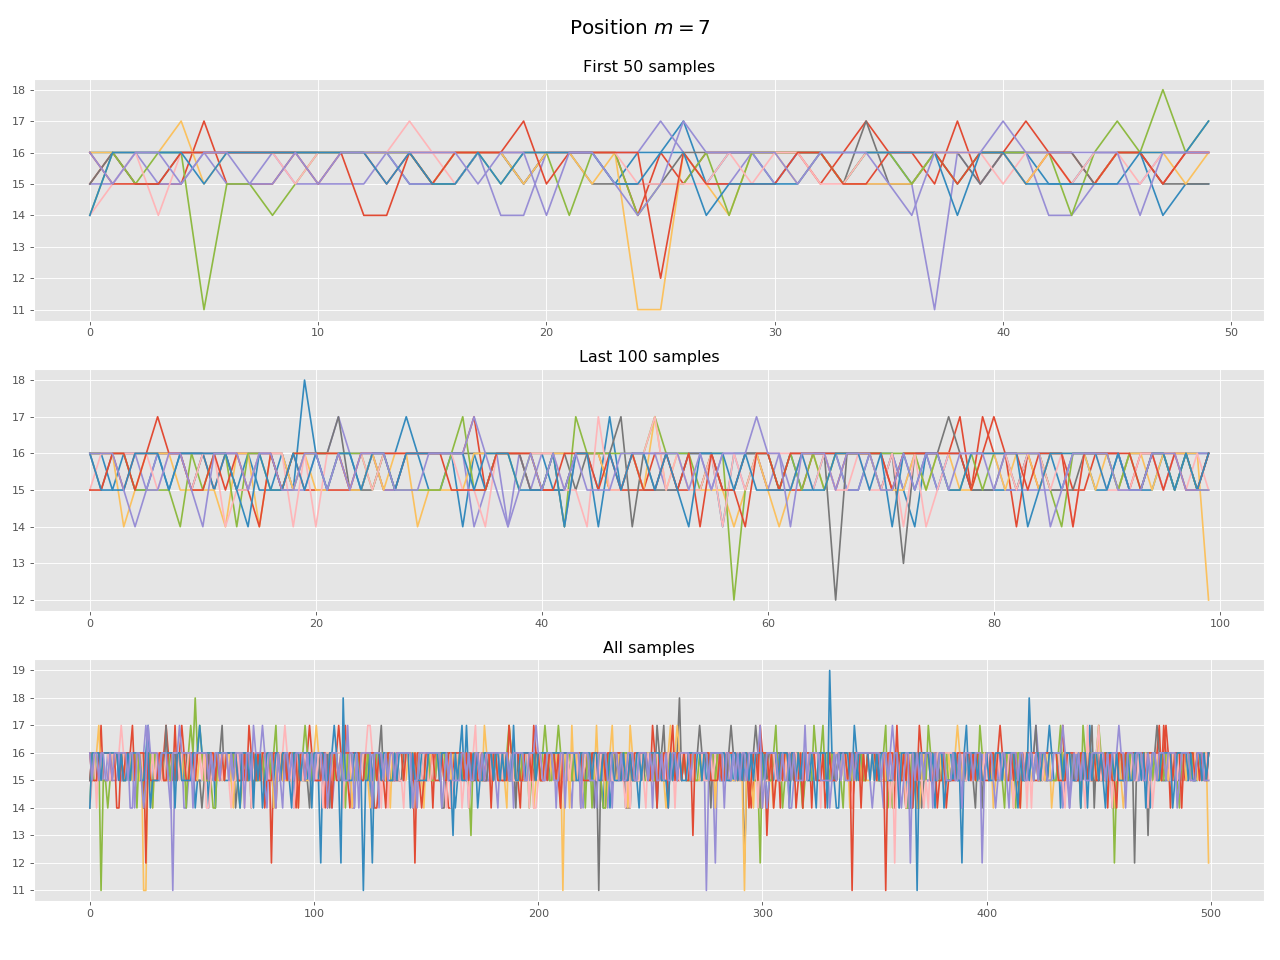
\includegraphics[width=.7\textwidth]{task4/figures/T_2_4/Q2/convergence_pos7.png}
			\caption*{Samples for position 7}
		\end{center}
	\end{figure}
	
	\begin{figure}[H]
		\begin{center}
			
			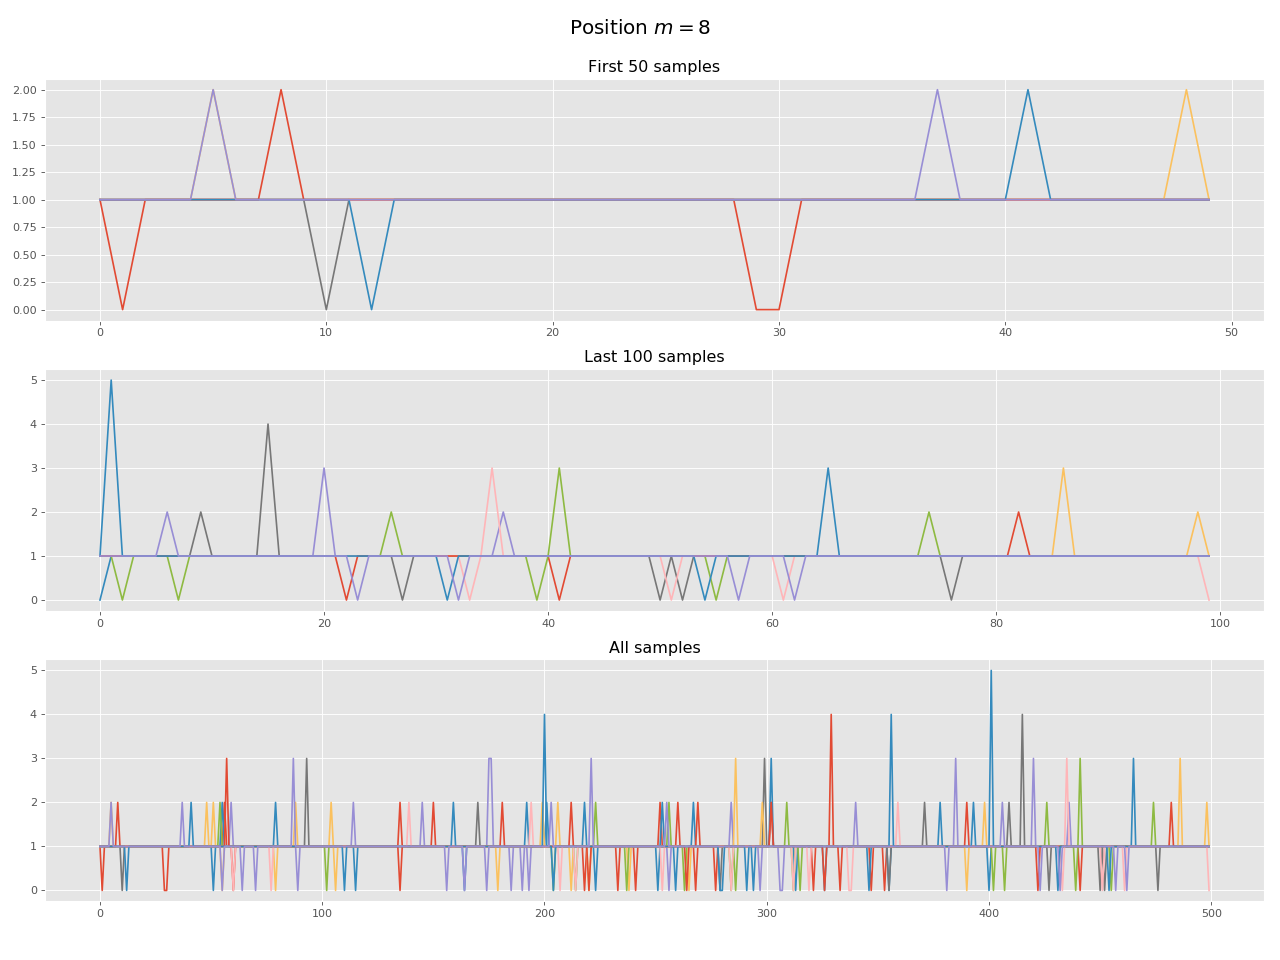
\includegraphics[width=.7\textwidth]{task4/figures/T_2_4/Q2/convergence_pos8.png}
			\caption*{Samples for position 8}
		\end{center}
	\end{figure}
	
	\begin{figure}[H]
		\begin{center}
			
			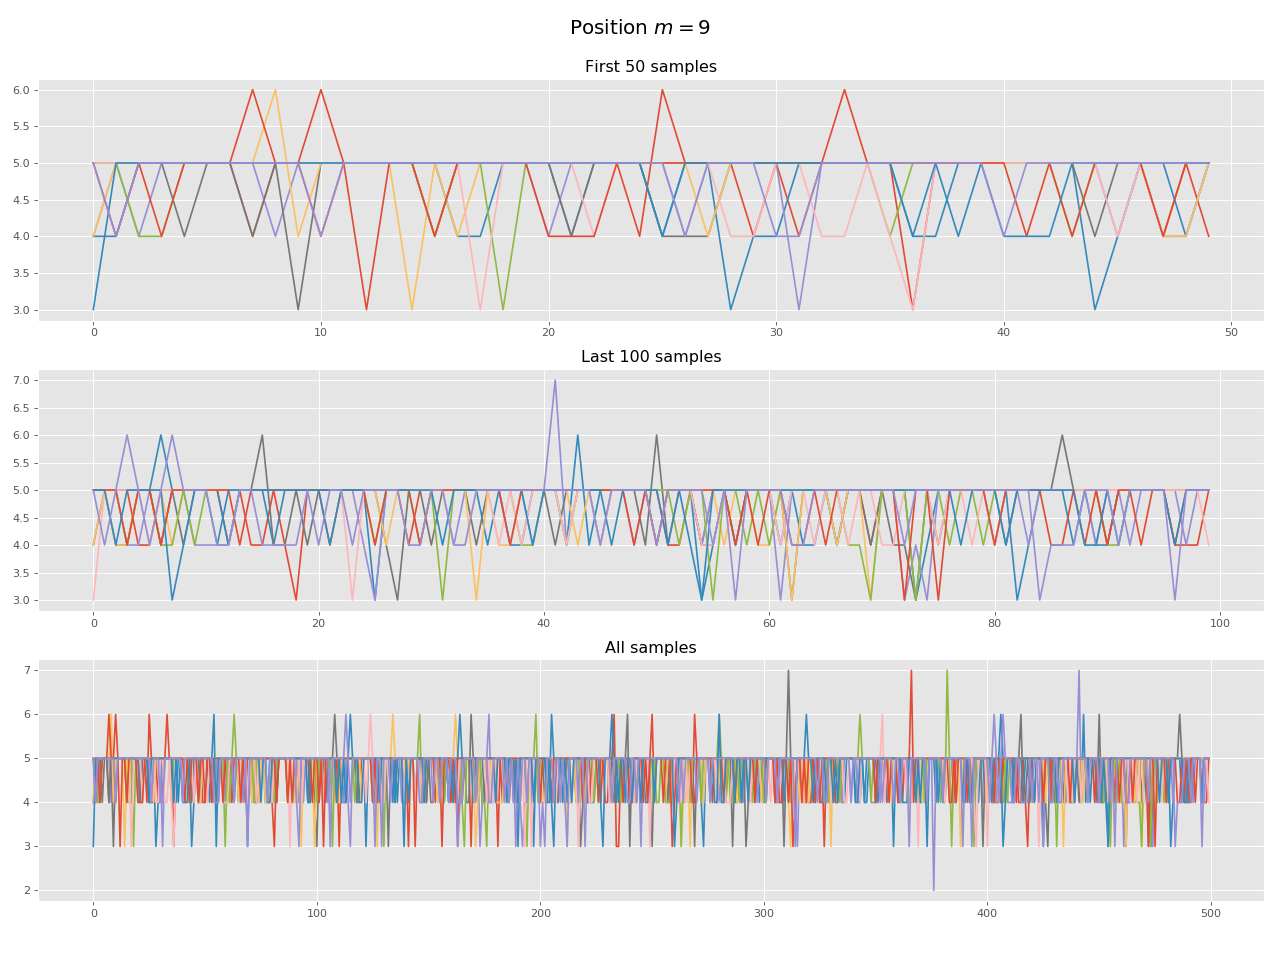
\includegraphics[width=.7\textwidth]{task4/figures/T_2_4/Q2/convergence_pos9.png}
			\caption*{Samples for position 9}
		\end{center}
	\end{figure}
	
	\newpage
	
	We can also observe the histograms to see the points around which the data gravitate to.
	
	\begin{figure}[H]
		\begin{center}
			
			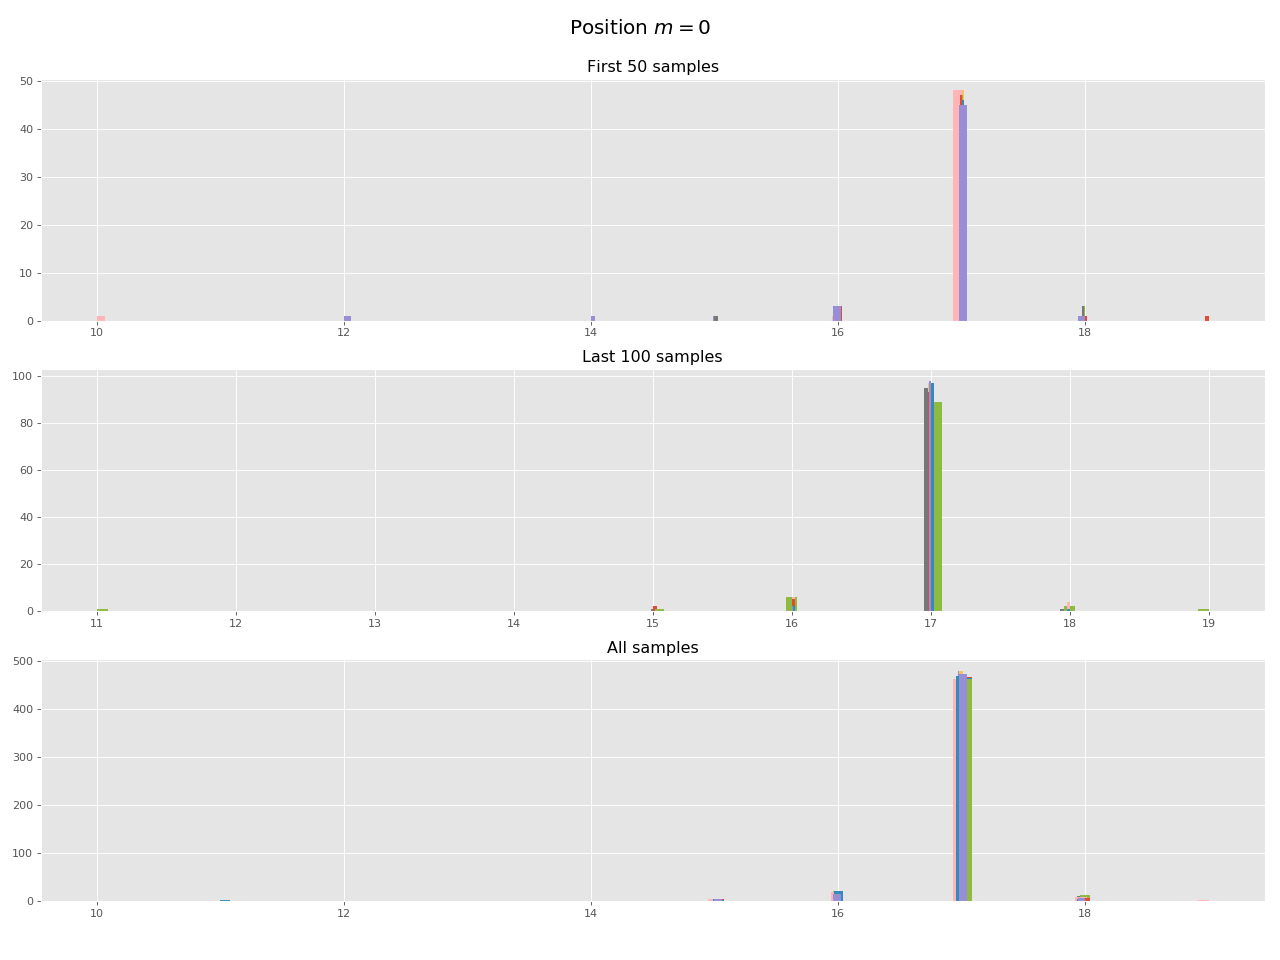
\includegraphics[width=.7\textwidth]{task4/figures/T_2_4/Q2/distribution_pos0.png}
			\caption*{Samples for position 0}
		\end{center}
	\end{figure}
	
	\begin{figure}[H]
		\begin{center}
			
			\includegraphics[width=.7\textwidth]{task4/figures/T_2_4/Q2/distribution_pos1.png}
			\caption*{Histogram for position 1}
		\end{center}
	\end{figure}
	
	\begin{figure}[H]
		\begin{center}
			
			\includegraphics[width=.7\textwidth]{task4/figures/T_2_4/Q2/distribution_pos2.png}
			\caption*{Histogram for position 2}
		\end{center}
	\end{figure}
	
	\begin{figure}[H]
		\begin{center}
			
			\includegraphics[width=.7\textwidth]{task4/figures/T_2_4/Q2/distribution_pos3.png}
			\caption*{Histogram for position 3}
		\end{center}
	\end{figure}
	
	\begin{figure}[H]
		\begin{center}
			
			\includegraphics[width=.7\textwidth]{task4/figures/T_2_4/Q2/distribution_pos4.png}
			\caption*{Histogram for position 4}
		\end{center}
	\end{figure}
	
	\begin{figure}[H]
		\begin{center}
			
			\includegraphics[width=.7\textwidth]{task4/figures/T_2_4/Q2/distribution_pos5.png}
			\caption*{Histogram for position 5}
		\end{center}
	\end{figure}
	
	\begin{figure}[H]
		\begin{center}
			
			\includegraphics[width=.7\textwidth]{task4/figures/T_2_4/Q2/distribution_pos6.png}
			\caption*{Histogram for position 6}
		\end{center}
	\end{figure}
	
	\begin{figure}[H]
		\begin{center}
			
			\includegraphics[width=.7\textwidth]{task4/figures/T_2_4/Q2/distribution_pos7.png}
			\caption*{Histogram for position 7}
		\end{center}
	\end{figure}
	
	\begin{figure}[H]
		\begin{center}
			
			\includegraphics[width=.7\textwidth]{task4/figures/T_2_4/Q2/distribution_pos8.png}
			\caption*{Histogram for position 8}
		\end{center}
	\end{figure}
	
	\begin{figure}[H]
		\begin{center}
			
			\includegraphics[width=.7\textwidth]{task4/figures/T_2_4/Q2/distribution_pos9.png}
			\caption*{Histogram for position 9}
		\end{center}
	\end{figure}
	
	We now see that the plots with high variance of samples have a few distinctive values that keep getting chosen in equal proportion.
	
	For a more quantitative overview of this method we can observe the convergence over the positions by using the estimated potential scale reduction statistics. This methods compares the variance of each position within each chain to its variance across chains.
	
	We will evaluate the convergence of our chain over time. For each time step we recompute the convergence from the beginning up until that point and then plot the convergence rate for each position from the second position until the end.
	
	\begin{figure}[H]
		\begin{center}
			
			\includegraphics[width=1\textwidth]{task4/figures/T_2_4/Q2/convergence_epsr.png}
			\caption*{Estimated potential scale reduction statistis over time}
		\end{center}
	\end{figure}
	
	We observe that the convergence happens under 100 samples.
	
	For accuracy we will introduce a metrics to evaluate how the performance of each chain changes over time. Since we are provided the true initial positions of the magic word we are estimating, we can compute the mean squared error for each sample.
	
	\begin{figure}[H]
		\begin{center}
			
			\includegraphics[width=1\textwidth]{task4/figures/T_2_4/Q2/mse_pos0.png}
			\caption*{MSE for position 0}
		\end{center}
	\end{figure}
	
	\begin{figure}[H]
		\begin{center}
			
			\includegraphics[width=1\textwidth]{task4/figures/T_2_4/Q2/mse_pos1.png}
			\caption*{MSE for position 1}
		\end{center}
	\end{figure}
	
	\begin{figure}[H]
		\begin{center}
			
			\includegraphics[width=1\textwidth]{task4/figures/T_2_4/Q2/mse_pos2.png}
			\caption*{MSE for position 2}
		\end{center}
	\end{figure}
	
	\begin{figure}[H]
		\begin{center}
			
			\includegraphics[width=1\textwidth]{task4/figures/T_2_4/Q2/mse_pos3.png}
			\caption*{MSE for position 3}
		\end{center}
	\end{figure}
	
	\begin{figure}[H]
		\begin{center}
			
			\includegraphics[width=1\textwidth]{task4/figures/T_2_4/Q2/mse_pos4.png}
			\caption*{MSE for position 4}
		\end{center}
	\end{figure}
	
	\begin{figure}[H]
		\begin{center}
			
			\includegraphics[width=1\textwidth]{task4/figures/T_2_4/Q2/mse_pos5.png}
			\caption*{MSE for position 5}
		\end{center}
	\end{figure}
	
	\begin{figure}[H]
		\begin{center}
			
			\includegraphics[width=1\textwidth]{task4/figures/T_2_4/Q2/mse_pos6.png}
			\caption*{MSE for position 6}
		\end{center}
	\end{figure}
	
	\begin{figure}[H]
		\begin{center}
			
			\includegraphics[width=1\textwidth]{task4/figures/T_2_4/Q2/mse_pos7.png}
			\caption*{MSE for position 7}
		\end{center}
	\end{figure}
	
	\begin{figure}[H]
		\begin{center}
			
			\includegraphics[width=1\textwidth]{task4/figures/T_2_4/Q2/mse_pos8.png}
			\caption*{MSE for position 8}
		\end{center}
	\end{figure}
	
	\begin{figure}[H]
		\begin{center}
			
			\includegraphics[width=1\textwidth]{task4/figures/T_2_4/Q2/mse_pos9.png}
			\caption*{MSE for position 9}
		\end{center}
	\end{figure}
	
	We observe that the error is gradually diminishing and converging to a specific value due to the reduction of the variance over time. Still for the positions on which the sampler remain indecisive such as position 1 and 4 the error remains high. 
	
	\newpage
	
	
	\section*{2.5 Stochastic volatility unknown parameter}
	
	Let us consider the problem presented in task 2.1. Now, we assume that the variance parameters $\sigma$ and $\beta$ are both unknown, while $\phi$ is given. The Bayesian setting is characterized by the priors:
	
	$$\sigma^2 \sim \mathcal{IG}(a=0.01, b=0.01)$$
	
	$$\beta^2 \sim \mathcal{IG}(a=0.01, b=0.01)$$
	
	Then, we obtain the posterior distributions of the variance parameters in closed form:
	
	$$ p(\sigma^2|\phi, x_{0:T}, y_{1:T}) = \mathcal{IG}(\sigma^2|a+\frac{T}{2}, b+\frac{1}{2}\sum_{t=1}^{T}(x_t-\phi x_{t-1})^2) $$
	
	$$p(\beta^2|\phi, x_{0:T}, y_{1:T}) = \mathcal{IG}(\sigma^2|a+\frac{T}{2}, b+\frac{1}{2}\sum_{t=1}^{T}e^{-x_t}y_t^2)$$
	
	\textbf{Code path} : ./Codes/task2.5  
	
	\subsection*{Question 13}
	
	We implemented a particle Gibbs sampler to compute the posterior distribution $p(\sigma^2, \beta^2|\phi, y_{1:T})$. To do so, at each iteration we alternatively sample from
	
	\begin{enumerate}
		
		\item[-] $p(\sigma^2|\phi, x_{0:T}, y_{1:t})$
		
		\item[-] $p(\beta^2|\phi, x_{0:T}, y_{1:t})$
		
		\item[-] $p(x_{0:T}|\theta, y_{1:T})$
		
	\end{enumerate}
	
	The initialization is perfomed considering as first value of $\sigma$ the true value, i.e., $\sigma = 0.1315$. In this problem, $\phi = 0.9709$. Then we sample the first values of $x_t$, for $t=0...T$, considering the distributions presented in task 2.1.
	
	
	Considering $N=10^4$ and $T=500$, with a $burn-in$ fase of 5000 iterations, we obtained the following marginal distributions for the variance parameters:
	
	\begin{center}
		
		\includegraphics[width=.4\textwidth]{task5/Gibbs_sigma2.jpeg}
		
		\includegraphics[width=.4\textwidth]{task5/Gibbs_beta2.jpeg}
		
	\end{center}
	
	
	
	\subsection*{Question 14}
	
	We tried to implement a Particle MCMC sampler for this model, by reusing the SMC implemented in 2.1, now modifed to become a Conditional SMC. 
	
	
	Our implementation works as follows: first we initialize $\sigma$ and $\beta$ to their correct values; then we initialize $x_{0:T}$ using the distributions given in task 2.1; we perform once the SMC (with resampling), and the output is a $(T+1) \times N$ matrix, that we need for the Conditional Sequential Monte Carlo.
	
	
	The sampling part has the following steps:
	
	\begin{enumerate}
		
		\item we sample $\sigma^2$ from $p(\sigma^2|\phi, x_{0:T}, y_{1:t})$;
		
		\item we sample $x_{0:T}$ running again the SMC algorithm, where  the $N^{th}$ particle's path is unchanged, with respect to the first SMC that we run. The sampling is performed by picking a random index $j$ in $\{1,...,N-1\}$ and considering the path of the $j^{th}$ particle;
		
		\item we sample $\beta^2$ from $p(\beta^2|\phi, x_{0:T}, y_{1:t})$.
		
	\end{enumerate}
	
	
	We obtained the following marginal distributions for the variance parameters:
	
	\begin{center}
		
		\includegraphics[width=.4\textwidth]{task5/CSMC_sigma2.jpeg}
		
		\includegraphics[width=.4\textwidth]{task5/CSMC_beta2.jpeg}
		
	\end{center}
	
	
	\subsection*{Question 15}
	
	As we can notice from the plots, our implementation does not work properly, since the marginal distributions provided are not the same. 
	
	
	Anyway, we provide the convergence rates for the two methods.
	
	
	Using Gibbs sampler, we obtain a trace that suits the one of an $Inverse Gamma$ for $\sigma^2$, but the one of $\beta^2$ corresponds to a $Gaussian$, as we can see in the following plots.
	
	\begin{center}
		
		\includegraphics[width=.4\textwidth]{task5/Gibbs_sigma2_convergence.jpeg}
		
		\includegraphics[width=.4\textwidth]{task5/Gibbs_beta2_convergence.jpeg}
		
	\end{center}
	
	
	Using CSMC, we obtain
	
	\begin{center}
		
		\includegraphics[width=.4\textwidth]{task5/CSMC_sigma2_convergence.jpeg}
		
		\includegraphics[width=.4\textwidth]{task5/CSMC_beta2_convergence.jpeg}
		
	\end{center}
	
	
	\newpage
	
	\section*{3.1 PyClone Light}
	
	In this problem, you should apply a collapsed Gibbs sampler in order to cluster mutations based on a Dirichlet Process Mixture Model (DPMM). The probabilistic model can, following the original publication, be described by the graphcal model in Figure 2(a), where $H$ is a Dirichlet Process (DP). We will instead use the grapical model in Figure 2(b), which yelds the same distribution when equipped with distributions as follows,
	
	
	\begin{equation}
	\begin{aligned}
	\pi &\sim \text{Gem}(\alpha) \\
	Z^n &\sim \pi \\
	\phi^k &\sim H_0 = \text{Beta}(1,1) \\
	b^n &\sim \text{Bin}(d^n, \phi^{Z^n})\\
	\end{aligned}
	\end{equation}
	
	\textbf{Code path} : ./Codes/task3.1  
	
	\subsection*{Question 16}
	
	Dirichlet process mixture models is a representative algorithm of the class of infinite mixture models with a non-parametric prior, a family of models that do not impose any a priori bound on $K$.
	
	The main idea is to have a method of working with an infinite amount of clusters which will be used to represent different distributions, which makes it a distribution over distributions. This can be done with a Dirichlet process, which can be in our case explaind with a stick-breaking construction. 
	
	The method generates a infinite sequence of numbers in range from $0$ to $1$, denoted with $\beta_k$ such that $ \beta \sim Beta(1,\alpha)$ for a arbitrary parameter $\alpha$. Beta values are then used to determinate the proportions of stick length as follows:
	
	$$ \pi_k = \beta_k \prod_{t=1}^{k-1} (1-\beta_t)$$
	
	Another common notation is:
	
	$$ \pi \sim GEM(\alpha) $$
	
	We can then compute $\theta_k$ as samples comming from different segments $\pi_k$ such that:
	
	$$ G(\theta) = \sum_{k=1}^{\infty} \pi_k \delta_{\theta_k}(\theta) $$
	
	where $\pi \sim GEM(\alpha)$ and $\theta \sim H$. Then once can show that G id distributed as a Dirichlet process with parameters $\alpha$ and a distribution $H$, i.e.$G \sim DP(\alpha,H)$.
	
	In our model sampled $\theta_k$ values correspond to $\phi_k$ probabilities of a successful outcome for a binomial distribution, with the number of trials being randomly generated for each sample. 
	
	Now we will derive the conditional probability for the next cluster placement which will be used in the collapsed Gibbs sampler.
	
	The probability of data point's cluster $z_i$ being a particular cluster $k$ is :
	
	$$ p(z_i = k \mid \mathbf{z}_{-i}, \mathbf{b}, \mathbf{d}, \theta, \alpha) \propto p(z_i = k \mid \mathbf{z}_{-i},\alpha) p(\mathbf{b}_i \mid \mathbf{b}_{-i}, \mathbf{d}, z_i = k, \mathbf{z}_{-i}, \theta ) $$
	
	Where we can write :
	
	$$ p(z_i \mid \mathbf{z}_{-i}, \alpha) = 
	\begin{cases}
	\frac{N_{k,-i}}{\alpha + N -1} \text{ if k has been seen before}\\
	\frac{\alpha}{\alpha + N -1} \text{ if k is a new cluster}\\
	\end{cases} $$
	
	
	First we will analyse the case if the cluster has been seen before. That means there are potentialy other points in observed data that are situated in the same cluster. We then procede to write:
	
	$$ p(\mathbf{b}_i \mid \mathbf{b}_{-i},\mathbf{d}, z_i = k, \mathbf{z}_{-i}, \theta ) = p(\mathbf{b}_i \mid \mathbf{b}_{-i,k}, \mathbf{d}_k, \theta ) = \frac{p(\mathbf{b}_i,\mathbf{b}_{-i,k} \mid \mathbf{d}_k,\theta )}{p( \mathbf{b}_{-i,k} \mid \mathbf{d}_k \theta )} $$ 
	
	$$ p(\mathbf{b}_i,\mathbf{b}_{-i,k} \mid \mathbf{d}_k,\theta ) = \int p(b_i\mid d_i,\phi^k) \left[ \sum_{j \neq i, z_j=k} p(b_j\mid d_j,\phi^k) \right] p(\phi^k \mid H_0) \text{d} \phi^k$$ 
	
	$$ p(\mathbf{b}_i,\mathbf{b}_{-i,k} \mid \mathbf{d}_k,\theta ) = \int Bin(b_i\mid d_i,\phi^k) \left[ \sum_{j \neq i, z_j=k} Bin(b_j\mid d_j,\phi^k) \right] Beta(\phi^k \mid a=1,b=1) \text{d} \phi^k$$ 
	
	
	Since the beta distribution is a conjugate prior to binomial distribution, we can write :
	
	$$ p(\mathbf{b}_i,\mathbf{b}_{-i,k} \mid \mathbf{d}_k,\theta ) = \binom{\sum_{z_j=k} d_j}{\sum_{z_j=k} b_j} \frac{B(\sum_{z_j=k} b_j + 1 , \sum_{z_j=k} d_j - \sum_{z_j=k} b_j +1)}{B(1,1)} $$ 
	
	
	
	Analogously :
	
	$$ p( \mathbf{b}_{-i,k} \mid \mathbf{d}_k \theta ) = \binom{\sum_{z_j=k,j \neq i} d_j}{\sum_{z_j=k,j \neq i} b_j} \frac{B(\sum_{z_j=k,j \neq i} b_j + 1 , \sum_{z_j=k,j \neq i} d_j - \sum_{z_j=k,j \neq i} b_j +1)}{B(1,1)} $$ 
	
	$$ p(\mathbf{b}_i \mid \mathbf{b}_{-i,k}, \mathbf{d}_k, \theta ) = \frac{\binom{\sum_{z_j=k} d_j}{\sum_{z_j=k} b_j} \frac{B(\sum_{z_j=k} b_j + 1 , \sum_{z_j=k} d_j - \sum_{z_j=k} b_j +1)}{B(1,1)}}{\binom{\sum_{z_j=k,j \neq i} d_j}{\sum_{z_j=k,j \neq i} b_j} \frac{B(\sum_{z_j=k,j \neq i} b_j + 1 , \sum_{z_j=k,j \neq i} d_j - \sum_{z_j=k,j \neq i} b_j +1)}{B(1,1)}} $$ 
	
	$$ p(\mathbf{b}_i \mid \mathbf{b}_{-i,k}, \mathbf{d}_k, \theta ) = \frac{\binom{\sum_{z_j=k} d_j}{\sum_{z_j=k} b_j}}{\binom{\sum_{z_j=k,j \neq i} d_j}{\sum_{z_j=k,j \neq i} b_j}} \frac{B(\sum_{z_j=k} b_j + 1 , \sum_{z_j=k} d_j - \sum_{z_j=k} b_j +1)}{B(\sum_{z_j=k,j \neq i} b_j + 1 , \sum_{z_j=k,j \neq i} d_j - \sum_{z_j=k,j \neq i} b_j +1)} $$ 
	
	For the case when the cluster was not observed before, i.e. it's a new cluster we have : 
	
	$$ p(\mathbf{b}_i \mid \mathbf{b}_{-i},\mathbf{d}, z_i = k^*, \mathbf{z}_{-i}, \theta ) = p(b_i \mid \theta ) = \int p(b_i\mid d_i,\phi^{k^*}) p(\phi^{k^*} \mid H_0) \text{d} \phi^{k^*} $$ 
	
	$$ p(b_i \mid \theta ) = \binom{d_i}{ b_i} \frac{B(b_i + 1 , d_i - b_i +1)}{B(1,1)} $$ 
	
	
	
	Finally we can put it all together to write:
	
	$$ p(z_i = k \mid ...) \propto      
	\begin{cases}
	\frac{N_{k,-i}}{\alpha + N -1}\frac{\binom{\sum_{z_j=k} d_j}{\sum_{z_j=k} b_j}}{\binom{\sum_{z_j=k,j \neq i} d_j}{\sum_{z_j=k,j \neq i} b_j}} \frac{B(\sum_{z_j=k} b_j + 1 , \sum_{z_j=k} d_j - \sum_{z_j=k} b_j +1)}{B(\sum_{z_j=k,j \neq i} b_j + 1 , \sum_{z_j=k,j \neq i} d_j - \sum_{z_j=k,j \neq i} b_j +1)} ...\\ 
	\text{ if k has been seen before}\\
	\\
	\\
	\frac{\alpha}{\alpha + N -1} \binom{d_i}{ b_i} \frac{B(b_i + 1 , d_i - b_i +1)}{B(1,1)} ... \text{ if k is a new cluster}\\
	\end{cases} $$

	
	
	\subsection*{Question 17}
	
	Our experiments will be run on our implementation of data generator. 
	
	The process of generating data starts by running the stick-breaking method to determinate the probabilities of picking each individual cluster. Next we sample $k$ different $\phi^k$ parameters for each of the clusters, from a beta distribution with parameters $a=1$ and $b=1$.
	We will use the sampled $\phi^k$ as probabilities of an action happening in the binomial distribution.
	
	When we want to sample our PyLight model for $N$ samples, we first decide what will be the cluster from which the data point will come. Then we generate the maximal number of trials for each sample, $d_i$ and finally sample our data point from a binomial distribution with parameters $d_i$ and $\phi^{z_i}$ where $z_i$ is the index of the cluster from which this data will be generated.  
	
	The next plot shows the placement of data points in the $b_i$, $d_i$ space colored by the true cluster.
	
	\begin{center}
		
		\includegraphics[width=.6\textwidth]{task6/figures/T_3_1/Q2/data_plot.png}
				
	\end{center}
	
	We draw $1000$ samples from the Gibbs sampler. The resulting Rand index and Mutual information plots suggest that the algorithm wasn't succesful in finding the right clusters for this model.
	
	\begin{center}
		
		\includegraphics[width=.6\textwidth]{task6/figures/T_3_1/Q2/rand_index.png}
		
		\includegraphics[width=.6\textwidth]{task6/figures/T_3_1/Q2/mutual_information.png}
		
	\end{center}	
	
	Further investigation shows that the number of cluster is decreasing over time, but at some point it stops in a local optima. Next plot shows the probabilities of a data point belonging to a specific cluster
	
	\begin{center}	
		\includegraphics[width=.6\textwidth]{task6/figures/T_3_1/Q2/sample_prob_0.png}
		
		\includegraphics[width=.6\textwidth]{task6/figures/T_3_1/Q2/sample_prob_18.png}
		
		\includegraphics[width=.6\textwidth]{task6/figures/T_3_1/Q2/sample_prob_42.png}
		
		\includegraphics[width=.6\textwidth]{task6/figures/T_3_1/Q2/sample_prob_64.png}
		

	\end{center}	
	
	
	Possible improvements could be made by making a better initialization rather then assigning a specific cluster to each point.
	
	\newpage
	
	
	\section*{3.2 Predicting a relation based on Indian Buffet Process}
	Let us suppose that we observe the interactions between a set of entities and we wish to extract informative representations that are useful for making predictions about the entities and their relationships. One basic challenge is link prediction, where we observe the relationships (or “links”) between some pairs of entities in a network (or “graph”) and we try to predict unobserved links. 
	
	In our model, each entity is described by a set of binary features. We are not given these features a priori and will attempt to infer them. We assume that the probability of having a link from one entity to another is entirely determined by the combined effect of all pairwise feature interactions. If there are $K$ features, then let $Z$ be the $N \times K$ binary matrix where each row corresponds to an entity and each column corresponds to a feature such that
	$$ 
	z_{ik} \equiv Z(i,k) = 
	\begin{cases}
	1 \text{\ \ \ if the $i^{th}$ entity has feature $k$} \\
	0 \text{\ \ \ otherwise}
	\end{cases}
	$$
	Let $Z_i$ denote the feature vector corresponding to entity $i$.
	
	Let $W$ be a $K \times K$ real-valued weight matrix where $w_{kk'} \equiv W(k, k')$ is the weight that affects the probability of there being a link from entity $i$ to entity $j$ if both entity $i$ has feature $k$ and entity $j$ has feature $k'$.
	
	Then the likelihood is defined as follows:
	$$
	Pr(y_{ij}=1|Z,W) = \prod_{i,j}Pr(y_{ij}|Z_i,Z_j,W)
	$$
	Given the feature matrix $Z$ and the weight matrix $W$, the probability that there is a link from entity $i$ to entity $j$ is
	$$
	Pr(y_{ij}=1|Z,W) = \sigma(Z_iWZ_j^T) = \sigma(\sum_{k,k'}z_{ik}z{jk'}w_{kk'}) 
	$$
	where $\sigma(\cdot)$ is a function that transforms values on $(-\infty, \infty)$ to $(0,1)$ such as the sigmoid function $\sigma(x) = (1+e^{-x})^{-1}$.
	
	Given the full set of observations $X$, we wish to infer the posterior distribution of the feature matrix $Z$ and the weight $W$.
	
	Without any prior knowledge about the features or their weights, a natural prior for $W$ is given by 
	$$
	w_{kl} \sim \mathcal{N}(0,\sigma^2).
	$$
	
	We generate the feature matrix $Z$ using the Indian Buffet Process. Each row of $Z$ corresponds to a diner at an Indian buffet; each column corresponds to a dish at the infinitely long buffet. If a customer takes a particular dish, then the entry that corresponds to the customer's row and the dish's column is a 1, otherwise the entry is 0. The first customer chooses a $Poisson(\alpha)$ number of dishes to sample; the $i^{th}$ customer tries each previously sampled dish with probability proportional to the number of people that have already tried the dish and then samples a $Poisson(\frac{\alpha}{i})$ number of new dishes. 
	
	We do inference implementing a MCMC sampler. At each iteration, we have to:
	\begin{enumerate}
		\item resample $Z$, given $W$;
		\item resample $W$, given $Z$.
	\end{enumerate}

	\textbf{Code path} : ./Codes/task3.2
	
	\subsection*{Question 19}
	In the algorithm implementation that we provide, at first we create a binary feature matrix $Z$, using the Indian Buffet Process. As previously mentioned, The first customer chooses a $Poisson(\alpha)$ number of dishes to sample. Then, for each custumer $i$ we perform the following steps:
	\begin{enumerate}
		\item [-] we compute the probability of visiting past dishes, given by $p = m_k/i$, where m is the number of customer that have already tried dish $k$;
		\item[-] sampling from a uniform distribution $\mathcal{U}(0,1)$, we either accept and set $z_{i,k}=1$ or reject the proposal;
		\item[-] we compute the number of new dishes visited by customer $i$, sampling from a $Poisson(\frac{\alpha}{i})$.
	\end{enumerate}
	Once $Z$ is built, we initialize the weight matrix $W$, using the fact that
	$$
	w_{kl} \sim \mathcal{N}(0,\sigma^2).
	$$
	Then, the MCMC sampler begins.
	\begin{enumerate}
		\item To sample from the distribution defined by the IBP, we need to compute the conditional distribution $P(z_{ik}=1|Z_{-i,k})$, where $Z_{-i,k}$ denotes the entries of $Z$ other than $z_{ik}$. We have that
		$$
		P(z_{ik}=1|Z_{-i,k}) = \frac{m_{-i,k}+\frac{\alpha}{K}}{N+\frac{\alpha}{K}}
		$$
		where $m_{-i,k}$ is the number of customers that have tried dish $k$, not including $i$.
		
		So, for each column $k$ if $m_{-i,k}$  is greater than 0 we set $z_{ik}=1$ with probability given by the equation just stated. Otherwise, we delete that column. At the end of row $i$, we add $Poisson(\frac{\alpha}{N})$ new columns that have ones in that row. 
		\item We sequentially resample each of the weights in $W$ that correspond to non-zero features (or dishes) and drop all weights that correspond to all-zero features. 
		
		We use a Metropolis-Hastings step for each weight in which we propose a new weight from a Normal distribution centered around the old one. Then, the probability of accepting $w_{new}$, when the current weight is $w_{old}$ is given by
		\begin{align*}
		a(w_{new}|w_{old}) & = \frac{p*(w_{new})}{p*(w_{old})} \frac{q(w_{old}|w_{new})}{q(w_{new}|w_{old})} \\
		& = \frac{p(D|w_{new})p(w_{new})}{p(D|w_{old})p(w_{old})} \frac{q(w_{old}|w_{new})}{q(w_{new}|w_{old})} \\
		& = \frac{\sum_{i,j}\sigma(z_{ik}z_{jk}w_{kk',new})}{\sum_{i,j}\sigma(z_{ik}z_{jk}w_{kk',old})}\frac{p(w_{new})}{p(w_{old})}\frac{q(w_{old}|w_{new})}{q(w_{new}|w_{old})}
		\end{align*}
		knowing that the prior over the weights is a $Gaussian$ centered in 0, with standard deviation $\sigma$, and the proposal of $w_{new}$ from $w_{old}$ is  $Gaussian$ centered in $w_{old}$, with standard deviation $\sigma$.
	\end{enumerate}
	
	\subsection*{Question 20}
	Running the algorithm with inizial parameters $N = 10$, $\alpha = 10$, $\sigma=0.5$ we have the following results.
	\\
	\begin{center}
		\includegraphics[width=8cm]{task7/output_initial_alpha10_sigma05_N10.jpeg}
	\end{center}
	As initial setting, $K=23$. After performing the MCMC sampler, we obtain
	\\
	\begin{center}
		\includegraphics[width=9cm]{task7/output_final_alpha10_sigma05_N10.jpeg}
	\end{center}
	with $K=31$, using $10^3$ iterations for the sampling. 
	
	
	\subsection*{Question 21}
	Considering more customers, for instance $N=20$, our algorithm provides the following results.
	
	As initial setting we have $K=37$. Initial and final feature matrices are:
	\begin{center}
		\includegraphics[width=.4\textwidth]{task7/output_initial_alpha10_sigma05_N20.jpeg}
		\includegraphics[width=.4\textwidth]{task7/output_final_alpha10_sigma05_N20.jpeg}
	\end{center}
	After the MCMC sampler we end up with $K=34$ features.
	
	Varying the number of data points in the IBP slightly increases the number of clusters. This is because every extra data point (customer) gives the matrix another chance to add more features (dishes) from the distribution $Poisson(\frac{\alpha}{N})$.
	
	Considering different values of $\alpha$, for instance $\alpha=5$, we have:
	\begin{center}
		\includegraphics[width=.4\textwidth]{task7/output_initial_alpha5_sigma05_N15.jpeg}
		\includegraphics[width=.4\textwidth]{task7/output_final_alpha5_sigma05_N15.jpeg}
	\end{center}
	and we end up with $K=19$.
	
	Setting $\alpha=15$, we have:
	\begin{center}
		\includegraphics[width=.4\textwidth]{task7/output_initial_alpha15_sigma05_N15.jpeg}
		\includegraphics[width=.4\textwidth]{task7/output_final_alpha15_sigma05_N15.jpeg}
	\end{center}
	We started with $K=43$ and ended up with $K=67$ features.
	
	We can conclude by saying that  $\alpha$ directly controls the total number of features and how readily features are added to the generated data. This is due to the fact that the number of new dishes added by the $i^{th}$ customer during the MCMC sampler is drawn directly from a $Poisson$ distribution parameterized by $\alpha$.
	
\end{document}

